\documentclass[a4paper]{amsart}

\usepackage[backend=biber, isbn=false, doi=false, url=false, style=numeric, sortcites=true, citestyle=numeric, giveninits=true]{biblatex}
\bibliography{bibliografia.bib}

%---------------------------------------
\usepackage{xfrac}
\usepackage{amssymb}
\usepackage{amsmath}
\usepackage{amsthm}
\usepackage{csquotes}
\usepackage{stmaryrd}
\usepackage{wrapfig}
\usepackage{xspace}
\usepackage{tikz}
\usetikzlibrary{cd}
\usetikzlibrary{calc}
\usepackage{adjustbox}
\usepackage{capt-of}
\tikzstyle{dot}=[inner sep=1pt, fill, black, circle, draw, minimum size = 5pt]
\tikzstyle{highlight}=[inner sep=1pt, draw=black, fill=white, circle, minimum size = 9pt]
%\usepackage{hyperref}
\usepackage[capitalise, noabbrev]{cleveref}
\usepackage{enumitem}
\setlist[itemize]{noitemsep}
\setlist[enumerate]{noitemsep}
\setlist[enumerate,1]{label = (\roman*)}
% notes for todos:
\newcommand{\gnote}[1]{{\color{red}GG: #1}}
\newcommand{\dnote}[1]{{\color{blue}DQ: #1}}


%% theorems and stuff

\newtheorem{theorem}{Theorem}
\newtheorem{proposition}[theorem]{Proposition}
\newtheorem{example}[theorem]{Example}
\theoremstyle{definition}
\newtheorem{definition}[theorem]{Definition}
\newtheorem{lemma}[theorem]{Lemma}
\newtheorem{corollary}[theorem]{Corollary}
\newtheorem*{conjecture}{Conjecture}
\let\romanenumerate\enumerate
\let\endromanenumerate\endenumerate


%%% logic operators
\DeclareMathOperator\ivee{\mathrel{\rotatebox[origin=c]{270}{$\geqslant$}}}
\DeclareMathOperator\bigivee{\rotatebox[origin=c]{270}{\scalebox{2}{$\geqslant$}}}
\newcommand\iexists{\overline{\exists}}

%%% logics, languages and signatures
\newcommand\fol{\mathtt{FO}}
\newcommand\dna{\mathtt{DNA}}
\newcommand\dnal[1]{\mathtt{#1}}
\newcommand\langFol{\mathcal{L}_{\fol}}
\newcommand\cpc{\mathtt{CPC}}
\newcommand\ipc{\mathtt{IPC}}
\newcommand\Fm{\mathcal{F}\mathit{m}}
\newcommand\Eq{\mathsf{Eq}}
\newcommand{\atoms}{\mathtt{Var}}
\newcommand{\formulas}{\mathcal{F}\mathit{m}}
\newcommand{\subst}{\mathsf{Subst}}
\newcommand{\atomsubst}{\mathsf{At}}
\newcommand{\admsubst}{AS}
\newcommand{\id}{\mathsf{id}}
\newcommand{\nat}{\mathbb{N}}
\newcommand\cqc{\mathtt{CQC}}
\newcommand\langCqc{\mathcal{L}_{\cqc}}
\newcommand\inqI{\mathtt{InqI}}
\newcommand\inqB{\mathtt{InqB}}
\newcommand\langInqB{\mathcal{L}_{\inqB}}
\newcommand\inqBQ{\mathtt{InqBQ}}
\newcommand\langInqBQ{\mathcal{L}_{\inqBQ}}
\newcommand\langpd{\mathcal{L}_{\pd}}
\newcommand\hinqBQ{\mathcal{H}\inqBQ}
\newcommand\langCl{\mathcal{L}_{!}}
\newcommand\langInqBQms{\mathcal{L}_{\iexists}}
\newcommand\langInqBQma{\mathcal{L}_{\forall}}

%% varieties and classes
\newcommand\vari{\mathcal{V}}
\newcommand\emp{\mathsf{E}}
\newcommand\nvari{\mathcal{V}^\uparrow}
\newcommand\uvari{\mathcal{U}^\uparrow}
\newcommand\inqint{\mathtt{Inq\Lambda}}
\newcommand\dvari{\mathbb{D}}
\newcommand\us{\texttt{US}}
\newcommand\ovari{\mathcal{X}}
\newcommand\class{\mathcal{C}}

\renewcommand{\restriction}{ {\upharpoonright} }

%% operators 
\newcommand{\val}[1]{\mathfrak{#1}}
\newcommand{\dashV}{\reflectbox{$\;\Vdash$}}
\newcommand{\core}{\mathsf{core}}
\newcommand{\dom}{\mathsf{dom}}
\newcommand{\depth}{\mathsf{depth}}
\newcommand{\width}{\mathsf{width}}
\newcommand{\height}{\mathsf{depth}}

\newcommand{\rank}{\mathsf{rank}}
\newcommand{\sol}{sol}
\newcommand{\truth}{\mathsf{Truth}}
\newcommand{\closure}{Cl}
\newcommand{\logic}{Log}
\newcommand{\homset}{\mathtt{Hom}}
\newcommand{\enset}{\mathtt{End}}
\newcommand{\horn}{\mathsf{Horn}}


%%%% New commands

\newcommand\at{\mathtt{AT}}
\newcommand{\espace}[1]{\mathfrak{#1}}
\newcommand{\clop}{\mathcal{C}}
\newcommand{\upset}{\mathcal{U}}
\newcommand{\IL}{\textbf{IL}}
\newcommand{\Esa}{\mathsf{Esa}}
\newcommand{\sem}[1]{\llbracket #1 \rrbracket}
\newcommand{\Log}{Log}
\newcommand{\Int}{\mathrm{Int}}
\newcommand{\Cl}{\mathrm{Cl}}
\newcommand{\PF}{\mathcal{PF}}
\newcommand{\CU}{\mathcal{CU}}
\newcommand{\Iso}{\mathcal{I}}

\newcommand{\comp}[1]{\overline{#1}}
%%%% END New commands



%these are shitty as they are not semantic
\newcommand{\cA}{\mathcal{A}}
\newcommand{\cB}{\mathcal{B}}
\newcommand{\cC}{\mathcal{C}}
\newcommand{\cD}{\mathcal{D}}
\newcommand{\cE}{\mathcal{E}}
\newcommand{\cF}{\mathcal{F}}
\newcommand{\cL}{\mathcal{L}}
\newcommand{\cU}{\mathcal{U}}
\newcommand{\cX}{\mathcal{X}}
\newcommand{\cM}{\mathcal{M}}
\newcommand{\calR}{\mathcal{R}}
\newcommand{\calU}{\mathcal{U}}
\newcommand{\calH}{\mathcal{H}}
\newcommand{\calK}{\mathcal{K}}
\newcommand{\bK}{\mathbf{K}}
\newcommand{\bQ}{\mathbf{Q}}
\newcommand{\bV}{\mathbf{V}}
\newcommand{\bC}{\mathbf{C}}
\newcommand{\fE}{\mathfrak{E}}
\newcommand{\fK}{\mathfrak{K}}
\newcommand{\fF}{\mathfrak{F}}
\newcommand{\fG}{\mathfrak{G}}
\newcommand{\fH}{\mathfrak{H}}
\newcommand{\fP}{\mathfrak{P}}
\newcommand{\fT}{\mathfrak{T}}
\newcommand{\fR}{\mathfrak{R}}
\newcommand{\fS}{\mathfrak{S}}

% these are good
\newcommand{\BA}{\mathsf{BA}}
\newcommand{\HA}{\mathsf{HA}}
\newcommand{\HArfsi}{\mathsf{HA_{RFSI}}}


\newcommand\dep{\mathop{=\!}\xspace}

\newcommand{\varopIdent}{\mathbb{I}}
\newcommand{\varopSub}{\mathbb{S}}
\newcommand{\varopProd}{\mathbb{P}}
\newcommand{\varopUltraProd}{\mathbb{P}_U}
\newcommand{\varopCore}{\mathbb{C}^\Sigma}
\newcommand{\varopISP}{\varopIdent\varopSub\varopUltraProd}
\newcommand{\varopISPP}{\varopIdent\varopSub\varopProd\varopUltraProd}

\newcommand{\coregen}[1]{#1_{CG}}
\newcommand{\coremodels}[1]{Mod^c(#1)}
\newcommand{\coregenmodels}[1]{\coregen{Mod^c}(#1)}
\newcommand{\coretheories}[1]{Log^c(#1)}
\newcommand{\corevDash}{\vDash^c}
\newcommand{\ncorevDash}{\nvDash^c}
\newcommand{\sigmamodels}[1]{Mod^\Sigma(#1)}
\newcommand{\sigmagenmodels}[1]{\coregen{Mod^\Sigma}(#1)}

\newcommand{\xbar}{\vec{x}}
\newcommand\MP{\mathtt{MP}}
\newcommand\US{\mathtt{US}}
\newcommand\AS{\mathtt{AS}}

\newcommand\langInqI{\mathcal{L}_{\ipc}^\otimes}
\newcommand\langInt{\mathcal{L}_{\ipc}}
\newcommand\langIntsta{\mathcal{L}_{\mathtt{CL}}}
\newcommand\langInqst{\mathcal{L}^\otimes_{\mathtt{CL}}}
\newcommand\langDep{\mathcal{L}_{\mathtt{Dl}}}

\newcommand{\Schm}{\mathsf{Schm}}

%--------------------------------------------------------------



\title{Esakia Duals of Regular Heyting Algebras}
\date{\today}
\author{Gianluca Grilletti}
\author{Davide Emilio Quadrellaro}
\email{grilletti.gianluca@gmail.com}
\email{davide.quadrellaro@helsinki.fi}
\address{Munich Centre for Mathematical Philosophy,	Munich, Germany}
\address{Department of Mathematics and Statistics, University of Helsinki, P.O. Box 68 (Pietari Kalmin katu 5), 00014 Helsinki, Finland}
\thanks{The authors would like to thank Nick Bezhanishvili for suggesting the main question studied in this work. We are also grateful to Fan Yang for many helpful comments on the subject of this paper. Davide Emilio Quadrellaro was supported by grant 336283 of the Academy of Finland and Research Funds of the University of Helsinki.}
\keywords{Heyting algebras, Esakia spaces, dependence logic, duality theory}
\subjclass[2020]{06D20, 03C05, 03B55}


\begin{document}
	
		\begin{abstract}
	   We investigate in this article regular Heyting algebras by means of Esakia duality. In particular, we provide some characterisations of Esakia spaces which are dual to regular Heyting algebras and we show that there are continuum-many varieties of Heyting algebras generated by regular Heyting algebras. We also study several logical applications of these classes of objects and we use them to provide novel topological completeness theorems for inquisitive logic, $\dna$-logics and dependence logic.
	\end{abstract}
\maketitle

	\section*{Introduction}
	
	A Heyting algebra is said to be \textit{regular} if it is generated by its subset of regular elements, i.e. elements $x$ which are identical to their double negation $\neg \neg x$. In this article we investigate regular Heyting algebra from the viewpoint of Esakia duality and we establish several connections to intermediate logics, inquisitive logic, dependence logic and  $\dna$-logic. We refer the reader to \cite{Ciardelli2011-CIAIL,Yang2016-YANPLO,bezhanishvili_grilletti_quadrellaro_2022} for an introduction to these three kinds of logical systems.
	
	Regular Heyting algebras have recently come to attention for their role in the algebraic semantics of inquisitive logic \cite{grilletti} and more generally of so-called $\dna$-logics \cite{Quadrellaro.2019,bezhanishvili_grilletti_quadrellaro_2022}. $\dna$-logics, for \textit{double negation on atoms}, make for an interesting generalisation of inquisitive logic which arises when considering translations of intermediate logics under the double negation map. More precisely, $\dna$-logics are those set of formulas $L^\neg$ which contain a formula $\phi$ whenever $L$ contains $\phi[\sfrac{\overline{\neg p}}{\overline{p}}]$, namely  the formula obtained by replacing simultaneously $p$ by $\neg p$ for any variable $p$. Such logics were originally introduced in \cite{Miglioli1989-PIESRO} and it was shown already in \cite{Ciardelli.2009} that inquisitive logic is a paradigmatic example of such logics. 
	
	
	Regular Heyting algebras also play a role in dependence logic. The connection between the team semantics of dependence logic and Heyting algebras was originally pointed out in \cite[\S 3]{Abramsky2009-ABRFIT} and it was later proved in \cite{quadrellaro2021intermediate} that suitable expansions of regular Heyting algebras provide an algebraic semantics to propositional dependence logic. It was shown later in \cite{nakov.quadrellaro} that such algebraic semantics, both for inquisitive, dependence and $\dna$-logics, are unique in the sense provided by a suitable notion of algebraizability for non-standard logics.
	

	In this article we supplement the previous work on the subject by investigating regular Heyting algebras from the perspective of duality theory. Firstly, in \cref{preliminaries}, we review Esakia duality and the previous results on inquisitive and $\dna$-logics. In \cref{topological.semantics} we use Esakia duality and results from \cite{bezhanishvili_grilletti_quadrellaro_2022}  to provide a topological semantics to $\dna$-logics, and also for inquisitive logic, which differs from the topological semantics based on UV-spaces considered in \cite{grilletti}. In \cref{sec.characterisation} we consider at length the main question of this article and we provide some characterisations of (finite)  Esakia spaces duals to (finite) regular Heyting algebras.  In \cref{morphism.characterisation} we give a first characterisation of finite regular Heyting algebras in terms of p-morphism, while in \cref{quotient.characterisation} we provide a necessary condition for an arbitrary Esakia space to be regular and we also give an alternative description of finite regular Esakia spaces. This characterisation allows us to consider a problem originally posed to us by Nick Bezhanishvili: \textit{how many varieties of Heyting algebras are generated by regular Heyting algebras?}\footnote{This question was posed to the authors in personal communication in 2019.} In \cref{cardinality.sublattice} we answer this question by showing that there are continuum-many of such varieties, complementing the result from \cite{bezhanishvili_grilletti_quadrellaro_2022} showing that the sublattice of  regularly generated varieties extending $\mathtt{ML}$ is dually isomorphic to $\omega+1$.  Finally, in \cref{dependence.logic}, we review the connection between inquisitive and dependence logic and we establish a topological completeness result for dependence logic.  We conclude the paper in \cref{conclusion} by highlighting some possible ideas of further research.
	
	\section{Preliminaries}\label{preliminaries}
	
	We recall in this section the preliminary notions needed later in the paper.  We review the algebraic semantics of intermediate and $\dna$-logics, the Esakia's duality between Heyting algebras and Esakia spaces and fix some notational conventions used throughout the paper. We refer the reader to \cite{Burris.1981,9783030120955, Zakharyaschev.1997, Johnstone} for a detailed presentation of these notions and results. 
	
	\subsection{Orders, Lattices, Heyting Algebras}
	For $(P,\leq)$ a partial order and $Q\subseteq P$ we indicate with $Q^\uparrow$ and $Q^\downarrow$ the upset and downset generated by $Q$ respectively, that is
	\begin{equation*}
	    Q^\uparrow = \{ p\in P  \mid  \exists q \in Q. q \leq p \}
	    \qquad
	    Q^\downarrow = \{ p\in P  \mid  \exists q \in Q.q \geq p  \}.
	\end{equation*}
	For $p\in P$, we write $p^\uparrow$ and $p^\downarrow$ for the sets $\{p\}^\uparrow$ and $\{p\}^\downarrow$ respectively.
	We call a set $Q$ such that $Q = Q^{\uparrow}$ an \emph{upset}, and similarly we call a set $R$ such that $R = R^{\downarrow}$ a \emph{downset}. Given a finite poset $P$, we define the depth $\depth(x)$ of an element $p\in P$ as the size of a maximal chain in $p^\uparrow\setminus\{p\}$. We define $\height(P):=\text{sup}\{\depth(p)+1 \mid p\in P  \}$ and $\width(P)$ as the size of the greatest antichain in $P$.
	
	A \emph{Heyting algebra} is a structure $(H,\land,\vee,\to,1,0)$ where $(H,\land,\vee,1,0)$ is a bounded distributive lattice and  $\to$ is a binary operation on $H$ such that for every $a,b,c\in H$ we have $a \leq b\to c$ if and only if $a \land b \leq c$. Henceforth, we will write $H$ to indicate a Heyting algebra (i.e., omitting the signature) for brevity.
	We use the symbol $\HA$ to indicate the class of all Heyting algebras. The class $\HA$ of Heyting algebras is \emph{equationally defined}, that is, a \emph{variety}. With a slight abuse of notation, we also use the notation $\HA$ to indicate the \emph{category of Heyting algebras}, whose objects are Heyting algebras and whose arrows are algebra homomorphisms.
	
	A \emph{Boolean algebra} $B$ is a Heyting algebra satisfying the equation $x=\neg \neg x$ for all $x\in B$. We write $\BA$ for both the class and the category of Boolean algebras. For any Heyting algebra $H$, we say that $x\in H$ is \emph{regular} if $x=\neg \neg x$ and we let $H_\neg:=\{x\in H \mid x=\neg \neg x \}$. One can verify that $H_\neg$ is a subalgebra of $H$ with respect to its $\{\land,\to,0,1  \}$-reduct and that it forms a Boolean algebra with join $x\dot{\lor}y:= \neg (\neg x\land \neg y) $. We say that a Heyting algebra is \textit{regular}, or \textit{regularly generated}, if $H=\langle H_\neg \rangle$. 
	
	We also recall that a variety of algebras is a class of structures which is closed under subalgebras $\mathbb{S}$, products $\mathbb{P}$, ultraproducts $\mathbb{P}_U$ and homomorphic images $\mathbb{H}$. We write $\mathbb{V}(\cC)$ for the least variety containing a class of algebras $\cC$. 
	
	
	\subsection{Esakia Duality}\label{subsection:esakia duality}
	
	We recall the Esakia duality between Heyting algebras and  Esakia spaces. We refer the reader to \cite{9783030120955} for more details on Esakia spaces and Esakia duality.
	
	Let $(X,\tau)$ be a topological space, we write $\mathcal{C}(X)$ for its collection of clopen subsets, i.e. subsets $U\subseteq X$ which are both open and closed in the $\tau$-topology. For ease of read, in the remainder of the paper we will omit the reference to the topology $\tau$ and simply write $X$ to indicate a topological space. If such notation is needed for a given space $X$, we then  write $\tau_X$ for the collection of its basic opens. %As we shall be dealing essentially with Stone spaces throughout this article, our focus will be mostly on clopens rather than simply open sets. 
	
	Recall that a topological space is \emph{totally disconnected} if its only connected components are singletons. A \emph{Stone space} is a compact, Hausdorff and totally disconnected space. Stone's duality states that the category of Stone Spaces with continuous maps is dually equivalent to the category of Boolean algebras with homomorphisms.
	
	Esakia duality provides an analogue of this result for Heyting algebras. We define Esakia spaces as follows. 
	
		\begin{definition}[Esakia Space]
		Let $\mathfrak{E}=(X,\leq)$ be a pair consisting of a topological space $X$ and a partial order $\leq$ over $X$. Then we say that $\mathfrak{E}$ is a \textit{Esakia Space} if:
		\begin{itemize}
			\item[(i)]  $X$ is a compact space;
			\item [(ii)] For all $x,y\in \espace{E}$ such that $x\nleq y$, there is a clopen upset $U$ such that $x\in U$ and $y\notin U$;
			\item[(iii)] If $U$ is a clopen set, then also $U^\downarrow$ is clopen.
		\end{itemize}
	\end{definition}
	
	\noindent Condition $(ii)$ in the definition above is called \textit{Priestley Separation Axiom}. Spaces satisfying conditions (i) and (ii) are called \textit{Priestley Spaces} \cite[\S 11]{pries}, hence every Esakia Space is also a Priestley space. Moreover, it can be also verified that every Esakia space is a Stone space. We write $\mathcal{CU}(\mathfrak{E})$ for the set of clopen upsets over $\mathfrak{E}$.
	
	We write $\Esa$ to indicate the class of Esakia spaces. In analogy with $\HA$, we can see $\Esa$ as a category whose objects are Esakia spaces.	A morphism between Esakia spaces is a map that preserves the topological structure, the order-theoretical structure and the relation between the two. We call these maps \emph{p-morphisms}.
	
	\begin{definition}[p-morphism]
	    Given Esakia spaces $\espace{E} = (X, \leq)$ and $\espace{E'} = (X',\leq)$, a \emph{p-morphism} $f: \espace{E} \to \espace{E'}$ is a continuous map satisfying the two following conditions:
	    \begin{enumerate}
	        \item For all $x,y \in \espace{E}$, if $x \leq y$ then $f(x) \leq f(y)$;
	        \item For all $x\in \espace{E}$ and $y' \in \espace{E'}$ such that $f(x) \leq y'$, there exists $y \in \espace{E}$ such that $x \leq y$ and $f(y) = y'$.
	    \end{enumerate}
	\end{definition}
	
	\noindent	Continuity and compactness of the space ensure that the preimage of a clopen in $\clop(\espace{E'})$ is contained in $\clop(\espace{E})$.	Additionally, the back and forth conditions ensure that the preimage of downsets of $\espace{E'}$ are again downsets of $\espace{E}$. We write $f:\fE\twoheadrightarrow \fE'$ when $f$ is a surjective p-morphism from $\fE$ to $\fE'$.
	
	Esakia spaces allows us to provide a duality for Heyting algebras, in the same spirit of the Stone duality for Boolean algebras or the Priestley duality for bounded distributive lattices.  To be more precise, Leo Esakia proved that the categories $\HA$ and $\Esa$ are dually equivalent.	Since they will play a major role in the rest of the paper, we recall what are the functors of this equivalence.
	
	Given a Heyting algebra $H$, a subset $F\subseteq H$ is a \textit{prime filter} if it is a filter and, if $x\lor y\in F$ then $x\in F$ or $y\in F$. Let $X_H=\PF(H)$ be the set of all prime filters over $H$, we can endow $X_H$ with a topology $\tau_H$, having as sub-basis the following family of sets:
	\[ \{ \phi(a) \,|\, a\in H \} \cup \{ \phi(a)^c \,| \, a\in H \} \]
	where  $\phi(a) = \{ F\in \PF(H) \,|\, a\in F \}$. Moreover, if we consider the standard inclusion order $\subseteq$ between prime filters, the ordered space $\espace{E}_H = (X_H, \tau_H, \subseteq)$ so obtained is an Esakia space: we call this the \emph{Esakia dual of $H$}. 
	
	On the other hand, if $\fE$ is an Esakia Space we can define the algebra $H_{\espace{E}}$ over the set $\CU(\fE)$ of clopen upsets of $\fE$:
	\begin{equation*}
	\begin{array}{r@{\hspace{.3em}}c@{\hspace{.3em}}l  @{\hspace{1.5em}}  r@{\hspace{.3em}}c@{\hspace{.3em}}l  @{\hspace{1.5em}}  r@{\hspace{.3em}}c@{\hspace{.3em}}l}
	U \land V &= & U \cap V
	&U \lor V &= & U \cup V
	&U \rightarrow V &= & ((U\setminus V)^\downarrow)^c
	\end{array}
	\end{equation*}	
	\noindent
	where $U^c$ denotes the complement of $U$ in $\espace{E}$. We shall also write $\overline{U}$ for  $(U^{\downarrow})^c$. The algebra $H_{\espace{E}}$ is an Heyting algebra, which we call the \emph{Esakia dual of $H$}. Esakia proved that these two maps are functorial and define an equivalence of categories, in particular the following holds with respect to objects.
	
	\begin{theorem}[Esakia]\label{theorem:esakiaDuality}
		For every Heyting algebra $H$, we have $H\cong H_{\mathfrak{E}_H}$. For every Esakia Space $\mathfrak{E}$, we have $\mathfrak{E}\cong \mathfrak{E}_{H_{\mathfrak{E}}}$.
	\end{theorem}


	\noindent 	At the level of arrows, we have the following correspondence:
	\begin{itemize}
		\item Given a homomorphism $f: H \to H'$ between two Heyting algebras, we define the p-morphism $\hat{f}: \espace{E}_{H'} \to \espace{E}_{H}$ by $\hat{f}(x) = f^{-1}[x]$; 
		\item Given a p-morphism $g: \espace{E} \to \espace{E'}$ between two Esakia spaces, we define the homomorphism $\hat{g}: H_{\espace{E'}} \to H_{\espace{E}}$ by $\hat{g}(U) = g^{-1}[U]$.
	\end{itemize}
	
	\noindent These mappings, together with the ones presented above, provides a full duality between the categories $\HA$ and $\Esa$.  We indicate with $\CU: \HA \to \Esa$ and $\PF: \Esa \to \HA$ the corresponding functors.
	
	When restricted to the finite setting, Esakia duality delivers a dual equivalence between finite Heyting algebras and finite Esakia spaces. Since an Esakia space $\espace{E}$ is a Stone space, in the finite case its topology is discrete. This allows to study finite Esakia spaces only in terms of their order-theoretic structure and to treat them simply as finite partial orders. 
	
	
	\subsection{Semantics for Intermediate Logics}
	\label{subsection:semanticsIntermediate}
	
	Heyting algebras and Esakia Spaces are closely connected to intermediate logics, i.e. logics which lie between intuitionistic and classical propositional logic. Let $\at$ be a (countable) set of atomic variables and consider the set of formulas $\langInt$ generated by the following grammar:
	\begin{align*}
	\phi ::= p \mid  \bot \mid \top \mid\phi\land\phi \mid \phi\lor \phi \mid  \phi \rightarrow \phi.
	\end{align*}
	
	\noindent We write $\ipc$ for intuitionistic logic and $\cpc$ for classical propositional logic. There is a standard way to interpret these formulas on Heyting algebras -- see e.g.  \cite[Sec. 7.3]{Zakharyaschev.1997}.  Given a Heyting algebra $H$ and a map $\mu: \at \to H$ (also called a \emph{valuation}), we can interpret formulas of $\langInt$ on $H$ inductively as follows:
	
	\begin{equation*}
	\begin{array}{r@{\hspace{.1em}}l @{\hspace{1em}}  r@{\hspace{.1em}}l @{\hspace{1em}}  r@{\hspace{.1em}}c@{\hspace{.1em}}l}	
	\llbracket p \rrbracket^{H,\mu} &= \mu(p)
	&\llbracket \bot \rrbracket^{H,\mu} &= 0 \\[0.5em]
	\llbracket \top \rrbracket^{H,\mu} &=  1  
	&\llbracket \phi \land \psi \rrbracket^{H,\mu} &= \llbracket \phi \rrbracket^{H,\mu} \land \llbracket \psi \rrbracket^{H,\mu} \\[0.5em]
	\llbracket \phi \rightarrow \psi \rrbracket^{H,\mu} &= \llbracket \phi \rrbracket^{H,\mu} \to \llbracket \psi \rrbracket^{H,\mu}
	&\llbracket \phi \lor \psi \rrbracket^{H,\mu} &= \llbracket\phi \rrbracket^{H,\mu} \vee  \llbracket\psi \rrbracket^{H,\mu}.
	\end{array}
	\end{equation*}
	\smallskip
	\noindent
	Given an Heyting algebra $H$, we say that a formula $\phi$ is \emph{valid on $H$} (in symbols $H \vDash \phi$) if for every valuation $\mu$ we have $\sem{\phi}^{H,\mu} = 1$.
	Given a class of Heyting algebras $\class$, we say that $\phi$ is \emph{valid on $\class$} (in symbols $\class \vDash \phi$) if $\phi$ is valid on every member of $\class$.
	We call the set of formulas valid on the class $\class$ the \emph{logic of $\class$} and we write $\Log(\class)$. When algebras and valuations are clear from the context, we simply write $\llbracket \phi \rrbracket$ in place of $\llbracket \phi \rrbracket^{H,\mu}$.
	
	It is well known that the logic of the class $\HA$ is the \emph{intuitionistic logic} $\ipc$. We say that a set of formulas $L$ in the signature $\langInt$ introduced above is an \emph{intermediate logic} if $\ipc\subseteq L\subseteq \cpc$  and, additionally, $L$ is closed under \emph{modus ponens} and uniform substitution. We shall write $L\vdash \phi$ when $\phi\in L$. A possibly surprising result is that not only $\ipc$, but \emph{every} intermediate logic is sound and complete with respect to a variety of Heyting algebras, see e.g. \cite{Zakharyaschev.1997}. 
	
	The previous result can be combined with Theorem \ref{theorem:esakiaDuality} to obtain a semantics based on Esakia spaces. Let $\espace{E}$ be an Esakia space and consider a map $\mu: \at \to \clop\upset(\espace{E})$, which we call a \emph{topological valuation}. As for Heyting algebras, we can define an interpretation of formulas of $\langInt$ based on \emph{clopen upsets} of $\espace{E}$: 
		\begin{equation*}
	\begin{array}{r@{\hspace{.1em}}l @{\hspace{1em}}  r@{\hspace{.1em}}l @{\hspace{1em}}  r@{\hspace{.1em}}c@{\hspace{.1em}}l}	
	\llbracket p \rrbracket^{\espace{E},\mu} &= \mu(p)
	&\llbracket \bot \rrbracket^{\espace{E},\mu} &= \emptyset \\[0.5em]
	\llbracket \top \rrbracket^{\espace{E},\mu} &=  \mathfrak{E} 
	&\llbracket \phi \land \psi \rrbracket^{\espace{E},\mu} &= \llbracket \phi \rrbracket^{^{\espace{E},\mu}} \cap \llbracket \psi \rrbracket^{\espace{E},\mu}  \\[0.5em]
	\llbracket \phi \rightarrow \psi \rrbracket^{\espace{E},\mu} &= \comp{\llbracket \phi \rrbracket^{\espace{E},\mu} \setminus \llbracket \psi \rrbracket^{\espace{E},\mu}}
	&\llbracket \phi \lor \psi \rrbracket^{\espace{E},\mu} &= \llbracket\phi \rrbracket^{^{\espace{E},\mu}} \cup  \llbracket\psi \rrbracket^{^{\espace{E},\mu}}.
	\end{array}
	\end{equation*}
\smallskip
	\noindent
	Notice that these are exactly the Heyting algebra operations of the dual algebra $H_{\espace{E}}$. Also, since finite Esakia spaces are exactly finite posets, thess semantic clauses correspond exactly to the standard Kripke semantics for intuitionistic logic. We say that a formula $\phi$ is valid on a space $\espace{E}$ (in symbols $\espace{E} \vDash \phi$) if for every valuation $\mu:\at \to \clop\upset(\espace{E})$ we have $\sem{\phi}^{\espace{E},\mu} = \espace{E}$. 	For a class $\mathcal{E}$ of Esakia spaces, we say that $\phi$ is valid on $\mathcal{E}$ (in symbols $\mathcal{E} \vDash \phi$) if $\phi$ is valid on every member of the class. We call the set of formulas valid on the class $\mathcal{E}$ the \emph{logic of $\mathcal{E}$} and we write  $\Log(\mathcal{E})$.\footnote{In the literature on intuitionistic logic, the term \emph{topological semantics} refers to a different semantics than the one presented here, one in which atomic formulas are assigned to \textit{opens} of an \textit{arbitrary} topological space $(X,\tau)$. We refer the reader to \cite{bezhanishvili2019semantic} for more information on the topic.}
	
	As a consequence of the results for classes of Heyting algebras, we have that the class $\Esa$ of all Esakia spaces is intuitionistic logic and that every intermediate logic is the logic of some class of Esakia spaces. Firstly, let us recall the correspondence between varieties of Heyting algebras and intermediate logics.	Let $L$ be an intermediate logic and $Var(L)=\{H\in \HA \mid H\vDash L \}$ the corresponding variety.	The algebraic completeness theorem for intermediate logics states that for any intermediate logic $L$, $L\vdash \phi $ if and only if $Var(L)\vDash \phi$.
	Conversely, if $\mathcal{V}$ is a variety of Heyting algebras, then the definability theorem of varieties of Heyting algebra tells us that $H\in\vari$ if and only if $H\vDash Log(\mathcal{V})$, where $ Log(\mathcal{V}) = \{ \phi\in\langInt \,|\, \mathcal{V}\vDash\phi  \}$ is the logic of $\mathcal{V}$.
	
	Using the Esakia duality and the semantics presented above, it follows that $H\vDash \phi$ if and only if $\mathfrak{E}_H\vDash \phi$. We can then translate the definability theorem and the algebraic completeness to the setting of Esakia spaces. To this end, we firstly define the concept corresponding to a variety of Heyting algebras: 	we say that a class of Esakia spaces $\mathcal{E}$ is a \textit{variety of Esakia spaces} if $\mathcal{E}$ is closed under p-morphic images, disjoint unions and closed upsets (see \cite[Lem. 3.4.11]{ 9783030120955}). These operations correspond through Esakia duality to the operations of subalgebras, products and homomorphic images respectively.

	Let $\Lambda(\HA)$ and $\Lambda(\ipc)$ be the complete lattice of varieties of Heyting algebras and the complete lattice of intermediate logics respectively (see \cite[Sec. 7.6]{Zakharyaschev.1997}). 	It is straightforward to show that the arbitrary intersection of varieties of Esakia spaces is again a variety, thus we have that the family of varieties of Esakia spaces $\Lambda(\Esa)$ forms a complete lattice too.\footnote{
	Admittedly, we are using an improper terminology (also adopted, e.g., in \cite[Sec. 7.6]{Zakharyaschev.1997}):
	varieties are proper classes, hence we cannot talk about the \emph{set} of all varieties nor about the \emph{lattice} of all varieties.
	A way to dispense of this problem is to instead consider a lattice consisting of \emph{equational theories}, that is, sets of algebraic identities defined by a class of algebras or spaces (see, e.g., \cite[Section 14]{Burris.1981} for an overview of this account).
	To simplify our presentation we abstract away from these issues and we maintain the terminology ``lattice of varieties''.} In analogy with the algebraic case, we define the two functions $Space: \Lambda(\ipc) \rightarrow  \Lambda(\Esa)$ and $Log: \Lambda(\Esa) \rightarrow  \Lambda(\ipc)$ as follows:
	\begin{align*}
	    Space(L)&= \{\mathfrak{E}\in \Esa \mid  \mathfrak{E}\vDash L  \};\\
	    Log(\mathfrak{\mathcal{E}})&=\{\phi\in\langInt \mid  \mathcal{E}\vDash \phi  \}.
	\end{align*}
	
	\noindent
	By looking at these maps in light of the duality between Heyting algebras and Esakia spaces, we readily obtain the following result, which establishes a version of completeness and definability for varieties of Esakia spaces.
	
	\begin{theorem}
		Let $L$ be an intermediate logic,  $\mathcal{E}$ a variety of Esakia Spaces, $\phi$ a formula and  $\mathfrak{E}$ an Esakia Space. Then we have the following:
		\begin{align*}
    		\phi \in L &\Longleftrightarrow Space(L)\vDash \phi; \\
    		\mathfrak{E}\in \mathcal{E} & \Longleftrightarrow \mathfrak{E}\vDash Log(\mathcal{E}).
		\end{align*}
	\end{theorem}

	Finally, Esakia duality can be lifted to the level of the lattice of varieties of Heyting algebras, and of the lattice of Esakia spaces. In particular, the maps
	\begin{equation*}
	\begin{array}{l@{\hspace{4em}}l}
	\overline{\PF}: \Lambda(\HA) \to \Lambda(\Esa)
	&\overline{\clop\upset}: \Lambda(\Esa) \to \Lambda(\HA) \\
	\overline{\PF}(\vari) =  \{ \espace{E}_H \mid  H\in \vari \}
	&\overline{\clop\upset}(\mathcal{E}) = \{ H_{\espace{E}} \mid  \espace{E} \in \mathcal{E} \}
	\end{array}
	\end{equation*}
	
	\begin{wrapfigure}{r}{6.3cm}		
		\adjustbox{scale=0.8,}{
			\begin{tikzcd}
				\Lambda(\HA) \arrow[rrddd, "Log"', bend right] \arrow[rrrr, "\mathcal{PF}", bend left] &  &                                                                 &  & \Lambda(\Esa) \arrow[llddd, "Log", bend left] \arrow[llll, "\mathcal{CU}"] \\
				&  &                                                                 &  &                                                                            \\
				&  &                                                                 &  &                                                                            \\
				&  & 	\Lambda(\ipc)^{op} \arrow[lluuu, "Var"'] \arrow[rruuu, "Space"] &  &                                                                           
		\end{tikzcd}}
	\end{wrapfigure}

 \noindent are inverse to each other.  The names $\overline{\PF}$ and $\overline{\clop\upset}$ indicate that these maps can be seen as liftings of the maps $\PF$ and $\clop\upset$ respectively to families of varieties. The lattices $\Lambda(\HA)$ and $\Lambda(\Esa)$ are then isomorphic, whence we also obtain that $\Lambda(\ipc)\cong^{op}\Lambda(\HA)\cong\Lambda(\Esa)$. The relations between the lattices $\Lambda(\HA)$, $\Lambda(\Esa)$  and $\Lambda(\ipc)$ are depicted in the diagram to the right, where arrows indicate lattice isomorphisms.
	


	\subsection{$\dna$-Logics}
	\label{subsection:dnaLogicsAndAlgebraicSemantics}
	
	In this paper, we are especially interested in regular Heyting algebras and their connection to Esakia spaces. This class of structures has important connections to a family of (non-standard) logics closely related to intermediate logics, i.e. \emph{$\dna$-logics}, from \textit{double negation on atoms}. These logics were originally introduced in \cite{Miglioli1989-PIESRO} and later studied in \cite{Ciardelli.2009,bezhanishvili_grilletti_quadrellaro_2022}. Notice that, for any formula $\phi$, we write $\phi[\sfrac{\overline{\neg p}}{\overline{p}}]$ for the formula obtained by replacing simultaneously $p$ by $\neg p$ for any atom $p$ occurring in $\phi$. 
	
	
	\begin{definition}
		For every intermediate logic $L$,  its \textit{negative variant} $L^\neg$ is defined as follows:
		$$ L^\neg \;=\; \{\,\phi\in\langInt \,|\, \phi[\sfrac{\overline{\neg p}}{\overline{p}}]\in L  \,\}.$$
		We call the negative variant of some intermediate logic a \emph{$\dna$-logic}.
	\end{definition}
	
	\noindent	Every $\dna$-logic contains the formula $\neg\neg p \to p$ for every atomic proposition $p\in\at$---but in general this is not true if we replace $p$  by an arbitrary formula $\phi$.
	So we can think of $\dna$-logics as intermediate logics where atoms do not play the role of \emph{arbitrary formulas}, since the principle of \emph{uniform substitution} does not hold, but rather the role of \emph{arbitrary negated formulas}. We notice that $\dna$-logics are an example of \textit{weak logics} in the sense of \cite[Def. 2]{nakov.quadrellaro}, i.e. they are consequence relations closed under permutations of atomic variables.
	
	Given a $\dna$-logic $\dnal{L}$ there is a standard way to find an intermediate logic $L$ such that $L^{\neg} = \dnal{L}$, as the following lemma shows.	
	\begin{lemma}
	    Given a $\dna$-logic $\dnal{L}$, define the set
	    \begin{equation*}
	        S(\dnal{L}) \;:=\; \{\, \phi \,|\, \sigma (\phi) \in \dnal{L} \text{ for every substitution $\sigma$} \,\}.
	    \end{equation*}
	    Then $S(\dnal{L})$ is an intermediate logic and $(S(\dnal{L}))^{\neg} = \dnal{L}$.
	\end{lemma}
	
	\noindent We refer the reader to \cite[Thm. 4.6]{bezhanishvili_grilletti_quadrellaro_2022} for the proof of the previous lemma. 	$S(\dnal{L})$ is usually referred to as the \emph{schematic fragment} of the logic $\dnal{L}$---see for example \cite{Ciardelli.2009}.
	
	
	There is also another way to characterize $\dna$-logics, that is, through their \emph{algebraic semantics} based on Heyting algebras.  	Let $H$ be a Heyting algebra, then  we call a valuation $\mu: \at \to H$ \emph{negative} if every atom is mapped to a regular element of $H$, or equivalently if $\neg\neg \mu(p) = \mu(p)$ for every $p$. If we restrict the algebraic semantics presented in Subsection \ref{subsection:semanticsIntermediate} to negative valuations we obtain a correct semantics for $\dna$-logics, in the following sense:
	If $H$ is a Heyting algebra, the set of formulas $\phi$ such that $\sem{\phi}^{H,\mu} = 1$ for every \emph{negative valuation} $\mu$ is a $\dna$-logic---we call this set the \emph{$\dna$-logic of $H$}. The notion of $\dna$-validity on algebras and classes of algebras are then defined as usual, but by considering only negative valuations.
	
	In \cite{bezhanishvili_grilletti_quadrellaro_2022} this semantics was employed in order to adapt results from the field of intermediate logic to study $\dna$-logics. In particular, we can show that $\dna$-logics form a lattice $\Lambda(\ipc^\neg)$, dual to a particular sublattice of $\Lambda(\HA)$. We write $ K \preceq H$ whenever $K$ is a subalgebra of $H$. 
	
	\begin{definition}[$\dna$-variety]\label{dna-variety}
	    A variety of Heyting algebras $\vari$ is called a \emph{$\dna$-variety} if it is additionally closed under the operation:
	    \begin{equation*}
	        \vari^{\uparrow} \;=\; \{\, H \mid \exists K\in \vari.\; K_{\neg} = H_{\neg} \text{ and } K \preceq H \,\}.
	    \end{equation*}
	\end{definition}
	
	\noindent We write $\dvari(\cC)$ for the smallest $\dna$-variety of algebras containing $\cC$. We let $\Lambda(\HA^{\uparrow})$ be the sublattice of $\Lambda(\HA)$ comprised of all and only the $\dna$-varieties. We remark here that, since $\dna$-varieties are uniquely determined by their regular elements, there is a one-to-one correspondence between $\dna$-varieties and varieties generated by regular Heyting algebras.	
	
	It can be shown \cite[\S 3.4]{bezhanishvili_grilletti_quadrellaro_2022} that for any $\dna$-logic $\mathtt{L}$ the set  $Var^{\neg}(\mathtt{L}) := \{ H \mid  \forall \phi \in \dnal(L).\; H\vDash^{\neg} \phi \}$ is a $\dna$-variety and that given $\vari$ a $\dna$-variety, the set  $Log^{\neg}(\vari) := \{ \phi \mid  \vari\vDash^{\neg} \phi \}$ is a $\dna$-logic. With these preliminary results in place, we can state the correspondence between $\dna$-logics and $\dna$-varieties, analogous to the one for intermediate logics and varieties. See \cite[Thm 3.35]{bezhanishvili_grilletti_quadrellaro_2022} for the proof of the following theorem. 
	\begin{theorem}
		The Lattices $\Lambda(\ipc^{\neg})$ and $\Lambda(\HA^{\uparrow})$ are dually isomorphic.
		In particular, the maps $Var^{\neg}$ and $Log^{\neg}$ are inverse to each other.
	\end{theorem}
	
	Usually, (propositional) inquisitive logic $\inqB$ is introduced, analogously to dependence logic, in terms of team semantics \parencite{Ciardelli2011-CIAIL,Yang2016-YANPLO}. However, it can also be considered as a $\dna$-logic. We start by recalling the definitions of the following intermediate logics:
	\begin{equation*}
	\begin{array}{l @{} l}
	\text{\texttt{KP} }	& = \space  \ipc \space + \space (\neg p \rightarrow q\lor r) \rightarrow (\neg p \rightarrow q) \lor (\neg p \rightarrow r) \\
	\text{\texttt{ND} }	& =\space  \ipc \space + \space \{ (\neg p \rightarrow \bigvee_{i\leq k} \neg q_i )\rightarrow \bigvee_{i\leq k}(\neg p \rightarrow \neg q_i) \mid k\geq 2 \}.
	\end{array}
	\end{equation*}
	
	\noindent Moreover, we define the intermediate logic $\mathtt{ML}$ as the set of all formulas which are valid in Kripke frames (i.e. posets) of the form $(\wp(n){\setminus}\emptyset, \supseteq)$ for $0<n<\omega$. We refer the reader to \cite{Zakharyaschev.1997} for more details on these systems. 	It is a well-known fact that $\mathtt{ND}\subseteq \mathtt{KP}\subseteq \mathtt{ML}$. The following theorem establishes an important connection between these intermediate logics and inquisitive logic.
	
	\begin{theorem}[Ciardelli \cite{Ciardelli.2009}]		
		Inquisitive logic is the negative variant of any intermediate logics $L$ such that $\mathtt{ND}\subseteq L\subseteq \mathtt{ML}$.
	\end{theorem}

	In the light of the previous theorem, the algebraic approach that we introduced  to study $\dna$-logics can be employed to study inquisitive logic as well, as it was done in \cite{bezhanishvili_grilletti_quadrellaro_2022}. In fact, such algebraic approach  	extends  the original work in \cite{grilletti} on the algebraic semantics of inquisitive logic. It was later shown in \cite{nakov.quadrellaro} that this algebraic semantics for $\inqB$ is unique, making $\inqB$ (like every $\dna$-logic) algebraizable in a suitable sense.  We conclude this section by referring the reader especially to \cite{Ciardelli2022-lp, ciardelli2018inquisitive, ciardelli2018inquisitive} for a detailed introduction to inquisitive logic and inquisitive semantics.
	
	
	\section{Topological Semantics for $\dna$-Logics} \label{topological.semantics}

	In the previous section we have seen how one can use Heyting algebras to provide an algebraic semantics to $\dna$-logics. In this section  we use Esakia duality to adapt these results to the topological setting, thereby obtaining a topological semantics for $\dna$-logics. As regular elements play a fundamental role in the algebraic setting, so the Stone space of maximal elements of an Esakia space plays a fundamental role in defining the topological semantics and the novel concepts used throughout this section. We thus start by introducing and studying the properties of this space.
	
	\subsection{The Stone Space of Maximal Elements}
	\label{subsection:stoneSpaceMaximalElements}
	We start by introducing and recalling some basic properties of regular clopens of Esakia spaces. These properties belong to the folklore, but we shall provide details of the proofs in these sections as it does not seem to us that they are explicitly present in the past literature. We stress however that \cref{hmap} is already stated in \cite[A.2.1]{9783030120955} and \cite[\S 3]{10.2307/20016257}.
	
	First, notice that given an Esakia space $\espace{E}$ we can consider two topologies on it:	the equipped Esakia topology $\tau_{\espace{E}}$ and the Alexandrov topology $\tau_\leq$ induced by the partial order on $\espace{E}$, i.e., the topology having as open sets the upsets according to the order. To distinguish the interior and closure operators in the two topologies we use the notations $\Int$, $\Cl$ and $\Int_{\leq}, \Cl_{\leq}$ respectively. In the rest of this article when we speak of regular subsets of an Esakia space we always mean \emph{regular sets under the order topology}.	
	\begin{definition}
		An upset $U$ of an Esakia space $\espace{E}$ is \textit{regular} if $\Int_{\leq}(\Cl_{\leq}(U)) = U$.
	\end{definition}	
	\noindent	We denote by $\mathcal{RCU}(\espace{E})$ the set of upsets of $\espace{E}$ that are (i) regular according to the Alexandrov topology and (ii) clopen according to the equipped Esakia topology. We start by providing several equivalent characterisation of such subsets.
	
	
	\begin{proposition}\label{regulars}
		Let $\fE$ be an Esakia space and let $U\in\mathcal{CU}(\fE)$.
		Then the following are equivalent:
		\begin{enumerate}
			\item $  U $ is regular;				
			\item $U=\overline{\overline{U}}$;				
			\item $U^\downarrow\setminus U   \;\subseteq\;   \overline{U}^\downarrow\setminus \overline{U}$.	
		\end{enumerate}
	\end{proposition}
	\begin{proof}
		Firstly, we notice that just by the definition of closure and interior we immediately obtain the following:
		\begin{align*}
			x\in \Int_{\leq}(\Cl_{\leq}(U))  \Longleftrightarrow x^\uparrow \subseteq U^\downarrow \Longleftrightarrow x\notin ((U^\downarrow)^c)^\downarrow \Longleftrightarrow x\in \overline{\overline{U}}.
		\end{align*}
		\noindent The equivalence between (ii) and (iii) is then proved as follows.	    
		\begin{description}
			\item[$(ii)\Rightarrow (iii)$] \medskip Suppose $U=\overline{\overline{U}}$ and let $x\in U^\downarrow\setminus U$.
			Since $x\notin U = (\overline{U}^{\downarrow})^c$, it follows that $x \in \overline{U}^{\downarrow}$.
			Moreover, since $x\in U^\downarrow$, we have that $x\notin ( U^\downarrow)^c = \overline{U}$.
			That is, $x\in  \overline{U}^\downarrow\setminus \overline{U}$.
			
			\item[$(iii)\Rightarrow(ii)$] Suppose that $U^\downarrow\setminus U \,\subseteq\, \overline{U}^\downarrow\setminus \overline{U}$ , we want to show that $U = (\overline{U}^{\downarrow})^c$. 
			
			($\subseteq$)
			Take $x \in U$ and consider any $y\geq x$, which lies again in $U$ since it is an upset.
			Since $U \cap \overline{U} = \emptyset$ it follows that $y \notin \overline{U}$;
			and since $y$ is an arbitrary element above $x$, it follows that $x\notin \overline{U}^{\downarrow}$, that is, $x \in (\overline{U}^{\downarrow})^c$.
			
			$(\supseteq)$
			Now suppose $x \in (\overline{U}^{\downarrow})^c$, which entails $x\notin \overline{U}^\downarrow \setminus \overline{U} $.
			Thus by assumption we have that $x\notin U^\downarrow \setminus U $.
			Then, either $x\in U$, which proves our claim, or $x\notin U^\downarrow$.
			However the latter gives a contradiction, since $x\in (U^\downarrow)^c = \overline{U}$ contradicts our assumption that $x\in  (\overline{U}^{\downarrow})^c \subseteq \overline{U}^c$.
			Hence we have that $x\in U$, which proves our claim. \qedhere
		\end{description}
	\end{proof}		
	
	\noindent	Now, given an upset $Q$ we indicate with $M(Q)$ the set of \emph{maximal} elements of $Q$, that is:
	\begin{equation*}
	M(Q)  \;:=\;  \{ q\in Q  \mid   \forall q' \in Q.( q' \geq q \implies q' = q )  \}.
	\end{equation*}
	
	\noindent We often write simply $M(p)$ in place of $M(p^\uparrow)$. We especially remark that, by compactness, it follows that for every Esakia space $\fE$ and for every element $x\in \fE$ the set $M(x)$ is nonempty -- see e.g. \cite[Thm. 3.2.1]{9783030120955}. An important characterisation of elements in $\mathcal{RCU}(\espace{E})$ is then in terms of the maximal elements of the Esakia space $\espace{E}$, as the following proposition makes precise. 
	
	\begin{proposition}\label{proposition:point condition regular upsets}
		Let $\fE$ be an Esakia space and $U\in\mathcal{CU}(\fE)$.
		Then the following are equivalent:
		\begin{enumerate}
			\item $U$ is regular;
			\item For every $x\in \espace{E}$ we have that $x\in U$ if and only if $ M(x)\subseteq U$.
		\end{enumerate}
	\end{proposition}	
	\begin{proof}
		Firstly notice that, if $x \in U$ then $M(x) \subseteq U$ since $U$ is an upset.
		So in particular $(ii)$ boils down to the right to left direction. We prove the two implications $(i) \Rightarrow (ii)$ and $(ii) \Rightarrow (i)$ separately.
		\begin{description}
			\item[$(i)\Rightarrow (ii)$]
			Given $x \in \espace{E}$, suppose that $M(x)\subseteq U$;
			we want to show that $x \in U$. Towards a contradiction, assume that $x\notin U$, which together with the previous assumption entails $x \in U^{\downarrow}\setminus U$.
			Since $U$ is regular by assumption, by Proposition \ref{regulars} it follows that $x\in \overline{U}^\downarrow\setminus \overline{U}$.
			Since $\overline{U}$ is an upset itself and there are maximal elements above every point of an Esakia space (this follows immediately by compactness, see \parencite[Thm. 3.2.1]{9783030120955}), it follows that $M(x) \cap \overline{U} \ne \emptyset$.
			But this is in contradiction with $M(x^{\uparrow}) \subseteq U$ since $U \cap \overline{U} = \emptyset$. We thus conclude that $x \in U$, as desired.
			
			\item[$(ii)\Rightarrow (i)$]
			By Proposition \ref{regulars}, it suffices to show that for an element $x \in \espace{E}$, if $x \in U^{\downarrow} \setminus U$ then $x \in \overline{U}^{\downarrow} \setminus \overline{U}$.
			So consider $x \in U^{\downarrow} \setminus U$.
			Since $x\notin U$, by assumption $M(x)\nsubseteq U$.
			By maximality of the elements in $M(x)$, we have that  $M(x)\nsubseteq U^\downarrow$, thus $M(x) \cap \overline{U} \ne \emptyset$.
			This implies that $x \in \overline{U}^{\downarrow}$.	Moreover, since  $x\in U^\downarrow$ we have that $x\notin \overline{U}$, thus concluding that $x \in \overline{U}^\downarrow \setminus \overline{U}$. \qedhere
		\end{description}
	\end{proof}
	
	By \cref{regulars} the elements of $\mathcal{RCU}(\mathfrak{E})$ correspond one-to-one to the regular elements of $H_{\espace{E}}$. In the light of this fact, it immediately follows that $ \mathcal{RCU}(\mathfrak{E}) $ is a Boolean algebra, where negation is defined as $\neg U:= \overline{U}$ and boolean disjunction as $U\dot{\lor} V:= \neg (\overline{U}\cap \overline{V})$. \cref{proposition:point condition regular upsets} suggests a connection between the Boolean algebras of regular elements and the \emph{Stone space of the maximal elements of $\espace{E}$}. Consider the set $M_{\espace{E}}$ of maximal elements of $\espace{E}$. It is well-known \cite[Thm. 3.2.3]{9783030120955} that this set forms a Stone space under the relative topology $\tau_{M_\espace{E}}$ inherited from $\espace{E}$:
	\begin{equation*}
	    U\in \tau_{M_\mathfrak{E}}  \;\Longleftrightarrow\;  \exists V \in \tau_{\mathfrak{E}} \text{ such that } U= V\cap  M_\mathfrak{E}.
	\end{equation*}
	
	\noindent The following lemma provides a correspondence between $\mathcal{RCU}(\espace{E})$ and $\cC(M_\espace{E})$. We attribute this theorem to Esakia, as it is mentioned in \cite[A.2.1]{9783030120955}, but we develop the proof idea contained in the remarks in \cite[\S 3]{10.2307/20016257}.
	
	\begin{theorem}[Esakia]\label{hmap}
		Let $\espace{E}$ be an Esakia space and $\mathcal{C}(M_{\espace{E}})$ the clopen sets of the Stone space $M_{\espace{E}}$.
		Then the map:	
		\begin{align*}
		M: & \: \mathcal{RCU}(\mathfrak{E}) \rightarrow	\mathcal{C}(M_\mathfrak{E}) \\
		M: & \: V \mapsto V \cap M_\mathfrak{E}
		\end{align*}
		\noindent is an isomorphism of Boolean algebras.
	\end{theorem}
	\begin{proof}
		%%% Well-defined
		First, we show that $M$ is a well-defined:
		let $V\in \mathcal{RCU}(\espace{E})$.
		Since $V$ is a clopen of $\espace{E}$, then $M(V) = V\cap M_\mathfrak{E}$ is a clopen of $M_{\espace{E}}$ by definition of the relative topology.
		
		%%% Homomorphism
		Secondly, we check that $M$ is a homomorphism.
		The only non-trivial case to check is the condition for negation.
		Let $U \in \mathcal{RCU}(\espace{E})$, then we have:
		\begin{equation*}
			M(\neg U) \;=\;
			M(\, \overline{U} \,) \;=\;
			M_\mathfrak{E} \cap (U^{\downarrow})^c \;=\;
			M_\mathfrak{E}\setminus M(U) \;=\;
			\neg M(U).
		\end{equation*}
		
		%%% Injective
		\noindent
		Thirdly, we show that $M$ is injective.
		Suppose $M(U) = M(V)$ for $U,V \in \mathcal{RCU}(\espace{E})$, then for any $x\in \espace{E}$ we have that $M(x)\subseteq U$ if and only if $M(x)\subseteq V$.
		So by Proposition \ref{proposition:point condition regular upsets} it follows that $x\in U$ if and only if $x\in V$, whence we obtain $U = V$.
		
		%%% Surjective
		Finally, we show that $M$ is surjective.
		Let $U\in \mathcal{C}(M_\espace{E})$, we want to find a $V\in \mathcal{RCU}(\espace{E})$ such that $M(V) = U$.  Now, since $U$ is a clopen of $M_{\espace{E}}$, by definition of the relative topology of $M_\fE$ we have that $U=V\cap M_\fE$ for some clopen $V\in \tau_\fE$. Then, since  taking downsets preserves being clopen, it follows that $V^\downarrow$ and $(V^c)^\downarrow$ are also clopen. Hence $Z=V^\downarrow\setminus (V^c)^\downarrow$ is clopen as well and, moreover $M(Z)=U$. Finally, as we have that $x\in V$ if and only if $x^\uparrow\subseteq U= M(Z)$ it follows by \cref{proposition:point condition regular upsets} that $Z$ is also regular. So we found an element $Z \in \mathcal{RCU}(\espace{E})$ which is mapped to $U$, thus proving that $M$ is surjective.
	\end{proof}
	
	\noindent The following corollary follows immediately using Stone's duality. Notice that, if $B$ is a Boolean algebra, we write $\fS_B$ for its dual Stone space.
	
	\begin{corollary}\label{stonemaxdual}
		Let $H$ be a Heyting algebra, then the Stone dual $\fS_{H_\neg}$ of the Boolean algebra $H_\neg $ is isomorphic to the Stone space $M_{\espace{E}_H}$, i.e. $ \fS_{H_\neg}\cong M_{\espace{E}_H}$.
	\end{corollary}
	\begin{proof}
		By Theorem \ref{hmap} we have that $\mathcal{RCU}(\espace{E}_H)\cong \mathcal{C}(M_{\espace{E}_H})$, and consequently $H_\neg\cong\mathcal{C}(M_{\espace{E}_H})$.
		By Stone duality it follows that $ \fS_{H_\neg}\cong M_{\espace{E}_H} $.
	\end{proof}
	
	
	\subsection{Topological Completeness}
	

	The results of \cref{subsection:stoneSpaceMaximalElements} suggest to define a semantics for $\dna$-logics in terms of Esakia spaces and regular clopen upsets. Given an Esakia space $\espace{E}$ we call a  function $\mu:\at\rightarrow \mathcal{RCU}(\espace{E})$ a \textit{$\dna$-valuation} over $\espace{E}$.
	For $\mu$ a $\dna$-valuation, define the interpretation of formulas over $\espace{E}$ as follows:
	
		\begin{equation*}
	\begin{array}{r@{\hspace{.1em}}l @{\hspace{1em}}  r@{\hspace{.1em}}l @{\hspace{1em}}  r@{\hspace{.1em}}c@{\hspace{.1em}}l}	
	\llbracket p \rrbracket^\mathfrak{\espace{E},\mu} &= \mu(p)
	&\llbracket \bot \rrbracket^\mathfrak{\espace{E},\mu} &= \emptyset \\[0.5em]
	\llbracket \top \rrbracket^\mathfrak{\espace{E},\mu} &=  \mathfrak{E}  
	&\llbracket \phi \land \psi \rrbracket^\mathfrak{\espace{E},\mu} &= \llbracket \phi \rrbracket^{\espace{E},\mu} \cap \llbracket \psi \rrbracket^\mathfrak{\espace{E},\mu}  \\[0.5em]
	\llbracket \phi \rightarrow \psi \rrbracket^\mathfrak{\espace{E},\mu} &= \overline{ \llbracket \phi \rrbracket^\mathfrak{\espace{E},\mu} \setminus \llbracket \psi \rrbracket^{\mathfrak{\espace{E},\mu}} }
	&\llbracket \phi \lor \psi \rrbracket^\mathfrak{\espace{E},\mu} &= \llbracket\phi \rrbracket^{\mathfrak{\espace{E},\mu}} \cup  \llbracket\psi \rrbracket^{\mathfrak{\espace{E},\mu}}.
	\end{array}
	\end{equation*}
	
	\smallskip
	
	\noindent
	The only difference with the definition of \cref{subsection:semanticsIntermediate} being that in the atomic case the interpretation is restricted to $\mathcal{RCU}(\espace{E})$.
	Notice however that not \emph{all} the formulas have to range over the set $\mathcal{RCU}(\espace{E})$. For example, it is not true in general that the union of two regular sets is regular, and in fact $\sem{p \vee q}^{\espace{E},\mu}$ may be a non-regular element of $\clop\upset(\espace{E})$. We then say that a formula $\phi$ is \emph{$\dna$-valid} on a space $\espace{E}$ ($\espace{E} \vDash^{\neg} \phi$) if $\sem{\phi}^{\espace{E},\mu} = \espace{E}$ for every $\dna$-valuation $\mu$. We say that a formula $\phi$ is $\dna$-valid on a class of spaces $\cE$ ($\cE \vDash^{\neg} \phi$) if it is $\dna$-valid on every element of the class. We write $Log^\neg(\cE)$ for the set of the $\dna$-valid formulas of $\cE$.
	
	In analogy with the algebraic case, we define a special family of varieties of Esakia spaces, closed under an additional operation which preserves the structure of the regular clopen upsets.
	
	\begin{definition}[$\dna$-variety of Esakia spaces]
	    A {$\dna$-variety of Esakia spaces} $\mathcal{E}$ is a variety of Esakia spaces additionally closed under the following operation:
	    \begin{equation*}
	        \mathcal{E}^{M} = \{ \espace{E} \mid  \exists \espace{F}\in \mathcal{E}.\; \exists f: \espace{E} \twoheadrightarrow \espace{F}.\; f\restriction M_{\espace{E}} \text{ is an isomorphism of Stone spaces}  \}.
	    \end{equation*}
	\end{definition}
	
	\noindent  Given a class $\cE$ of Esakia spaces, we write $\mathbb{S}(\cE)$ for the smallest $\dna$-variety of Esakia spaces containing $\cE$. The connection between $\dna$-varieties of algebras and $\dna$-varieties of spaces follows immediately from \cref{stonemaxdual}.  We then obtain that the family of $\dna$-varieties of Esakia spaces forms a sublattice of $\Lambda(\Esa)$, which we write as $\Lambda(\Esa^{M})$. When we restrict Esakia duality to $\dna$-varieties of Heyting algebras and $\dna$-varieties of Esakia spaces, we immediately obtain the following theorem.
	\begin{theorem}
	    The maps $\overline{\PF}$ and $\overline{\clop\upset}$ restricted to the sublattices $\Lambda(\HA^{\uparrow})$ and $\Lambda(\Esa^{M})$ induce an isomorphism of the two lattices.
	\end{theorem}
	\begin{proof}%[Proof sketch]
	    Notice that, given $H$ and $K$ Heyting algebras dual to $\espace{E}$ and $\espace{F}$ respectively, the two conditions
	    \begin{itemize}
	        \item[(i)] $ K_{\neg} = H_{\neg} \text{ and } K \preceq H $;
	        \item[(ii)]$ \exists f: \espace{E} \twoheadrightarrow \espace{F}.\; f^{-1}: \mathcal{RCU}(\espace{F}) \to \mathcal{RCU}(\espace{E}) \text{ is a Boolean algebras isomorphism}$;
	    \end{itemize}
	    \noindent are dual to each other. By Theorem \ref{stonemaxdual} the latter is equivalent to:
	    \begin{itemize}
	    	\item[(iii)] $\exists f: \espace{E} \twoheadrightarrow \espace{F}.\; f\restriction M_{\espace{E}} \text{ is a homeomorphism of Stone spaces}$.
	    \end{itemize}
	    \noindent  Given this, it is immediate to verify the main statement.	    
	\end{proof}
	
	\noindent Combining this statement with the algebraic completeness for $\dna$-logics we obtain that $\Lambda(\ipc^{\neg})\cong^{op}\Lambda(\HA^{\uparrow}) \cong \Lambda(\Esa^{M})$, which establishes the completeness of this topological semantics with respect to $\dna$-logics. Given a $\dna$-logic $ \mathtt{L}$ we write $Space^{\neg}(\mathtt{L}) $ for the $\dna$-variety of Esakia spaces which validates all formulas in $\mathtt{L}$. The previous observation translates to the following theorem. 
	
	\begin{theorem}\label{algebraic.completeness.dna}	
	Let $\mathtt{L}$ be a $\dna$-logic,  $\mathcal{E}$ a $\dna$-variety of Esakia Spaces, $\phi$ a formula and  $\mathfrak{E}$ an Esakia Space. Then we have the following:
		\begin{align*}
    		\phi \in \mathtt{L} &\Longleftrightarrow Space^{\neg}(\mathtt{L})\vDash^\neg \phi; \\
    		\mathfrak{E}\in \mathcal{E} & \Longleftrightarrow \mathfrak{E}\vDash^\neg Log^{\neg}(\mathcal{E}).
		\end{align*}
	\end{theorem}
	
This also delivers a topological semantics for inquisitive logic which differs from the one previously studied in \cite{grilletti}, rather based on UV-spaces. Since inquisitive logic $\inqB$ is the negative variant of any intermediate logic between $\mathtt{ND}$ and $\mathtt{ML}$, the former result shows that inquisitive logic also admits a topological semantics based on Esakia spaces, which mirrors its algebraic semantics based on regular Heyting algebras. 
\begin{corollary}
	Let $L$ be any intermediate logic between $\mathtt{ND}$ and $\mathtt{ML}$, then:
	\[ \phi\in \inqB \Longleftrightarrow  Space^{\neg}(L)\vDash^\neg \phi.      \]
\end{corollary}


	\section{Regular Esakia Spaces}\label{sec.characterisation}

	In the algebraic semantics of $\dna$-logics, a central role is played by regular Heyting algebras, as the interpretation of any formula in a Heyting algebra under a $\dna$-valuation lies in the subalgebra generated by its regular elements. More precisely, every $\dna$-variety is generated by its regular elements \cite{bezhanishvili_grilletti_quadrellaro_2022}, thus motivating the key role of regular Heyting algebras in the study of $\dna$-logics. 
	
	It is actually possible to give a stronger version of this result. We recall that a Heyting algebra is \textit{subdirectly irreducible} if it has a second greatest element. A class of Heyting algebras $\class$ has the \textit{$\dna$-finite model property} if $\class\nvDash^\neg \phi$ whenever $H\nvDash^\neg  \phi$ for some finite $H\in \class$. The $\dna$-version of the finite model property for classes of Esakia spaces is defined analogously. Since we will always consider the $\dna$-semantics defined above, we shall simply refer to this property as the finite model property. The relation between this notion and the standard one was investigated in \cite[\S 4.4]{bezhanishvili_grilletti_quadrellaro_2022}. The following results were proven in  \cite{bezhanishvili_grilletti_quadrellaro_2022}. \newpage
	\begin{theorem}\label{birkhoff} $\;$
		\begin{enumerate}
			\item Every $\dna$-variety of Heyting algebras $\cX$ is generated by its collection of regular, subdirectly irreducible elements: $\cX = \dvari(\cX_{RSI}) $.			
			\item If a $\dna$-variety $\cX$ has the finite model property, then it is generated by its finite, regular, subdirectly irreducible elements, i.e., $\cX=\dvari(\cX_{RFSI}) $.
		\end{enumerate}		
	\end{theorem}
	
	 It is then natural to use Esakia duality to obtain an analogue of the previous theorem for $\dna$-varieties of Esakia spaces. We say that $\fE$ is \textit{strongly rooted} if it has a least element $r$ such that $\{ r \}$ is open.  It is well-known that a Heyting algebra is subdirectly irreducible if and only if its dual Esakia space is strongly rooted (see \cite[p. 152]{esakia1979theory} and \cite[Thm. 2.9]{bezhanishvili2008profinite}). To extend the previous theorem to Esakia spaces we also need a notion dual to that of a regular Heyting algebra.
	
	\begin{definition}
		An Esakia space $\fE$ is \textit{regularly generated}, or simply \textit{regular}, if $H_\mathfrak{E}= \langle  (H_{\mathfrak{E}})_\neg \rangle $.
	\end{definition}
	
	\noindent Given an Esakia space $\fE$, we also write $\mathfrak{E}_r$ for the Esakia space dual to $\langle (H_{\mathfrak{E}})_\neg \rangle$. The following corollary follows then immediately from Esakia duality and \cref{birkhoff}.
	
	\begin{corollary}\label{birkhoff2} $\;$
		\begin{itemize}
			\item Every $\dna$-variety of Esakia spaces $\cE$ is generated by its collection of regular, strongly rooted elements: $\cE = \mathbb{S}(\cE_{RSI}) $.			
			\item If a $\dna$-variety $\cE$ has the finite model property, then it is generated by its finite, rooted, regular elements, i.e., $\cE=\mathbb{S}(\cE_{RFSI}) $.
		\end{itemize}		
	\end{corollary}
	
	
	Although the former corollary provides us with some information on $\dna$-varieties of Esakia space, the notion of regular Esakia spaces has so far received only an \textit{external} characterisation, as it was defined exactly in terms of its dual Heyting algebra. In this section we shall consider \textit{the problem of providing an internal characterisation of the class of regular Esakia spaces}.
	
	We give two partial answers to this question. Firstly, in \cref{morphism.characterisation}, we characterise regular Esakia spaces in terms of special p-morphisms, and we apply it to the finite case to obtain a more fine-grained description. Secondly, in \cref{quotient.characterisation}, we follow an alternative approach in term of quotient operations.  This allows us to obtain a necessary condition for an Esakia space to be regular, and also a particularly nice description of finite regular posets.
	
	
	\subsection{A Characterisation by Regular-Preserving Morphisms} \label{morphism.characterisation}
	
	One way to characterise regular Heyting algebras is to look at homomorphisms fixing the Boolean algebra of regular elements and homomorphisms fixing the subalgebra induced by it. When considering the topological duals of these operations, this motivates the following definitions. 
	
	\begin{definition} Let $h:\mathfrak{E}\rightarrow \mathfrak{E}'$ be a p-morphism, then
	\begin{itemize} 
	    \item \emph{$h$ preserves regulars} if $ h^{-1}: \mathcal{RCU}(\mathfrak{E}')  \to \mathcal{RCU}(\mathfrak{E})$ is an isomorphism of Boolean algebras;
	    \item \emph{$h$ preserves polynomials of regulars}  if  $ h^{-1}: \langle \mathcal{RCU}(\mathfrak{E}') \rangle \to \langle \mathcal{RCU}(\mathfrak{E})\rangle$ is an isomorphism of Heyting algebras. 
	\end{itemize}
	\end{definition}
	
	\noindent As regular clopen-upsets of Esakia spaces correspond to maximal elements, it follows that regular preserving p-morphisms can be characterised in terms of their action on maximal points. 
	
	\begin{proposition}\label{maximalinjectivity}
		Let $h:\mathfrak{E}\rightarrow \mathfrak{E}'$ be a p-morphism, then $h$ preserves regulars if and only if $h\restriction M_\mathfrak{E}$ is injective on maximal elements.
	\end{proposition}
	\begin{proof}
	$(\Rightarrow)$ Consider two distinct $x,y\in M_{\mathfrak{E}}$, since $M_{\mathfrak{E}}$ is a Stone space there are two disjoint clopen neighbourhoods $U_x, U_y$ of $x$ and $y$ respectively. From Theorem \ref{hmap} and Proposition \ref{regulars} it follows that  $M^{-1}(U_x)\cap M^{-1}(U_y) = \emptyset $. Now, since $h$ preserves regulars, it follows that $h^{-1}{\restriction}\mathcal{RCU}(\mathfrak{E}') $ is an isomorphism, whence $M^{-1}(U_x)= h^{-1}(V_x)$ and $M^{-1}(U_y)= h^{-1}(V_y)$ for some $V_x,V_y\in \mathcal{RCU}(\mathfrak{E}')$ such that $V_x\cap V_y=\emptyset$. Then, it follows that $h(x)\in V_x$ and $h(y)\in V_y$, whence $h(x)\neq h(y)$.
	
	$(\Leftarrow)$ Analogous to the previous direction.
	\end{proof}
	
	\noindent It is then immediate to conclude that extensions of a Heyting algebra with the same Boolean core of regular elements induce a surjective p-morphism of the dual spaces which is injective on maximal elements. 
	
	\begin{corollary}\label{corolla}
	    Suppose $A,B \in \HA$ and $A\preceq B$, $A_\neg=B_\neg$, then there is a continuous surjective p-morphism $h:\fE_B\twoheadrightarrow \fE_A$ which is also injective on maximal elements.
	\end{corollary}
	\begin{proof}
		By Esakia duality, the inclusion $A\preceq B$ induces a p-morphism $h:B_\fE\twoheadrightarrow A_\fE$ defined  by $h: F \mapsto F\cap A$,  where $F\subseteq B$ is any prime filter over $B$. The fact  that $h$ is continuous and surjective already follows from the duality between subalgebras and quotient spaces. By Proposition \ref{maximalinjectivity} above we also have that $h$ is injective on maximal elements.
	\end{proof}
	
	\noindent The following theorem provides a first characterisation of regular Esakia spaces.
	
		\begin{theorem}\label{theoremregular}
	The following are equivalent, for any Esakia Space $\mathfrak{E}$:
	\begin{enumerate}
	     \item $H_{\mathfrak{E}}$ is regularly generated;
	    \item $\forall K [ K\preceq H_{\mathfrak{E}}\text{ and }  (H_{\mathfrak{E}})_\neg=K_\neg  \text{ entail }  K= H_{\mathfrak{E}} ]$;
	    \item $\forall \mathfrak{E}', \forall f:\mathfrak{E}\twoheadrightarrow \mathfrak{E}' \; [\text{if } f{\restriction}  M_\mathfrak{E}\text{ is a homeomorphism, then  f is a homeomorphism}]$.
	\end{enumerate}
	\end{theorem}
	\begin{proof}
	Claims (i) and (ii) are equivalent by the definition of being regularly generated. We show the equivalence of (ii) and (iii).
	
	$(ii)\Rightarrow (iii)$ Let $ f:\mathfrak{E}\twoheadrightarrow \mathfrak{E}'$ be a surjective p-morphism, then by Esakia duality we have that $f^{-1}[H_{\mathfrak{E}'}]\preceq H_{\mathfrak{E}}$. By the same argument, if  $f\restriction  M_\mathfrak{E}$ is a homeomorphism, then $f^{-1}\restriction\mathcal{C}(M_{\mathfrak{E}'})$ is an isomorphism of Boolean algebras. It follows by Theorem \ref{hmap} that $f^{-1}: \mathcal{RCU}(\mathfrak{E}') \rightarrow \mathcal{RCU}(\mathfrak{E})   $ is also an isomorphism of Boolean Algebras, and by duality we have $\mathcal{RCU}(\mathfrak{E})=(H_{\mathfrak{E}})_\neg$ and $\mathcal{RCU}(\mathfrak{E}')=(H_{\mathfrak{E}'})_\neg$. It follows that $(f^{-1}[H_{\mathfrak{E}'}])_\neg=f^{-1}[(H_{\mathfrak{E}'})_\neg]= (H_{\mathfrak{E}})_\neg$, which by (ii) entails  $f^{-1}[H_{\mathfrak{E}'}]=H_{\mathfrak{E}}$. By duality it follows that $f$ is injective and  so $f:\mathfrak{E}\twoheadrightarrow\mathfrak{E}'$ is a homeomorphism.
	
	$(iii)\Rightarrow (ii)$ Let $K\preceq H_{\mathfrak{E}}$ be such that $K_\neg = (H_{\mathfrak{E}})_\neg$. By Corollary \ref{corolla}, there is a surjective p-morphism $h:\fE\twoheadrightarrow \fE_K$ which is also injective on maximal elements and such that $h(F)=F$ whenever $F$ is a prime filter over $K$. Hence, $h{\restriction}  M_\mathfrak{E}$ is a homeomorphism of Stone Spaces and by (iii) $h:\mathfrak{E}\twoheadrightarrow \fE_K$ is a homeomorphism of Esakia Spaces. By Esakia duality, it follows that $K= H_{\mathfrak{E}}$.
	\end{proof}
	
	In the finite context the characterisation of the previous theorem can be further strengthened. We recall the following definitions of  $\alpha$-reductions and $\beta$-reductions \cite{de1966connection, bezhanishvili2006lattices}, which are special p-morphisms of discrete Esakia spaces.
	
	\begin{definition}
	    Let $\fF$ be a partial order.
	    \begin{itemize}
	        \item  Suppose $x,y\in \fF$ are such that $x^\uparrow=y^\uparrow \cup \{x\}$. An \emph{$\alpha$-reduction} is a surjection $h:\fF\to \fF\setminus\{y\}$ such that $h(x)=h(y)$ and $h(z)=z$ whenever $z\neq y$.
	        \item  Suppose $x,y\in \fF$ are such that $x^\uparrow\setminus \{x\}=y^\uparrow\setminus\{y\}$. A \emph{$\beta$-reduction} is a surjection $h:\fF\to \fF\setminus\{y\}$ such that $h(x)=h(y)$ and $h(z)=z$ whenever $z\neq y$.
	    \end{itemize}
	\end{definition}	
	\noindent Notice that, since $\alpha$-reductions and $\beta$-reductions are not necessarily continuous with respect to the Stone topology of an Esakia space, we have introduced them only with respect to partial orders and not for Esakia spaces in general. This explains why we will use them to characterize only finite regular Esakia spaces, whose underlying topology is discrete.  In particular, in the finite case we can always look at immediate successors of points a poset: given any $x\in\fF$, we let $S(x):=\{ y\in \fF \mid  x<y \text{ and } x< z\leq y \Rightarrow z=y  \}$.  We then prove the following theorem characterising finite, regular posets.
	
\begin{theorem}\label{characterisation1}
	$H$ is a finite regular (subdirectly irreducible) Heyting algebra if and only if $\fE_H$ is a finite (rooted) poset such that:
	\begin{itemize}
		\item[(i)] For all non-maximal $x\in \fE_H$, $|S(x)|\geq 2$.		
		\item[(ii)] For all non-maximal $x,y\notin \fE_H$, if $x\neq y$, then $S(x)\neq S(y).$
	\end{itemize}
\end{theorem}
	\begin{proof}
		It suffices to consider conditions (i) and (ii) since it is already well-known that finite (subdirectly irreducible) Heyting algebras correspond to finite (rooted) posets under Esakia duality. 
		
		$(\Rightarrow)$	(i) If this is not the case, then there is a point $x\in \fE_H$ such that $S(x)=\{y\}$. Then,  we can apply the $\alpha$-reduction $h$ such that $h(x)=h(y)$ and $h(z)=z$ for all $z\neq x$. Then $h$ is a p-morphism which is injective on maximal elements, hence, by \cref{theoremregular} $h$ is an isomorphism, contradicting $x\neq y$, $h(x)=h(y)$. (ii) If this is not the case, then there are two distinct $x,y\in\mathfrak{E}$ such that $S(x)=S(y)$. We then apply the $\beta$-reduction $h$ such that $h(x)=h(y)$ and $h(z)=z$ for all $z\neq y$. But then $h$ is a  p-morphism which is injective on maximal elements, hence by \cref{theoremregular}, $h$ must also be an isomorphism, which gives us a contradiction.		
		
		$(\Leftarrow)$ If $H$ is not regular, then $\langle H_\neg \rangle \preceq H$ and $\langle H_\neg \rangle \neq H$. By  \cref{corolla} there exists a p-morphism $h: \fE_H\twoheadrightarrow \mathfrak{E}_{\langle H_\neg \rangle}$ which is also injective on maximal elements. Moreover, since $\langle H_\neg \rangle \neq H$, we also have that $\fE_H\neq \mathfrak{E}_{\langle H_\neg \rangle}$, meaning that $h\neq id$. Since  $\fE_H$ is finite, it follows that we can decompose $h$ into $\alpha$-reductions and $\beta$-reductions -- see  \cite[Prop. 3.1.7]{bezhanishvili2006lattices}. Hence $h=f_0\circ\dots\circ f_n$, where each $f_i$ for $i\leq n$ is either an $\alpha$- or a $\beta$-reduction. In particular, $f_n$ is an $\alpha$- or a $\beta$-reduction over  $\fE_H$, meaning that either (i) or (ii) holds.
	\end{proof}
	
	\subsection{A Characterisation by Quotients} \label{quotient.characterisation}
		
	We say that a poset (or Kripke frame) is \textit{compact} if for every element $x\in\fF$ there is maximal element $y\geq x$. In this section we shall introduce several equivalence relations over compact posets, and use them to provide a further characterisation of (finite) regular Esakia spaces.
		
	We notice in particular that, if $\fE$ is an Esakia space, then its order-reduct is a compact poset, since in Esakia spaces every point sees some maximal element. However, a  compact poset is not necessarily \textit{representable}, i.e. it is not necessarily isomorphic to the poset of prime filters of a Heyting algebra---we refer the reader to \cite[Appendix A.5]{9783030120955} and \cite{ BEZHANISHVILI2021107959} for more information on the representability of posets.

	The reason for working with compact posets is that, by means of some suitable equivalence relations that we introduce, we are able to give a necessary condition to establish if an infinite Esakia space is regular. In the finite case, where posets and Esakia spaces coincide, we obtain an additional description of finite, regular posets.  In particular, even though \cref{characterisation1} already provides a purely order-theoretic description of such posets, this second description makes more explicit how finite regular posets are controlled by their maximal elements. We start by considering the simpler case of inquisitive logic.   	
	
	\subsubsection{Strongly Regular Posets}\label{strongly.regular.inquisitive}
	
	We start by remarking that, in the case of inquisitive logic, we already have a classification of the posets dual to finite, regular, subdirectly irreducible inquisitive algebras. 
	
	In fact, by \cite[Cor. 4.12]{grilletti} it follows that these are the posets dual to Heyting algebras of the form $Dw^+(2^n)$ for $n<\omega$, where $Dw^+(X)$ is the collection of non-empty downsets of a poset $X$, and $2^n$ refers to the Boolean algebra $\wp(n)$. 	By taking prime filters over such algebras, it then readily follows that the finite, regular, rooted, inquisitive posets are exactly the Medvedev's frames, i.e. the posets  of the form $(\wp(n){\setminus}\{\emptyset \},\supseteq)$ for $n<\omega$. This motivates the following definition.
	
	\begin{definition}[Strongly Regular Poset]
		We say that a compact poset $\fF$ is \emph{strongly regular} if $M(x)\neq M(y)$ whenever $x\neq y$, $x,y\in \fF$. 
	\end{definition}
	
	\noindent In particular, we say that an Esakia space $\fE$ is strongly regular if its order-theoretic reduct is strongly regular.	
	
	From the characterisation of finite, regular, rooted, inquisitive posets that we recalled above it is easily seen that such posets are strongly regular: If $x$ and $y$ are different elements of $\wp(n){\setminus}\{\emptyset \}$, it follows (without loss of generality) that $m\in x\setminus y$ for some $m<n$, whence $x\supseteq \{m  \}$ but $y\nsupseteq \{m  \}$.
	
	Using the disjunctive normal form of inquisitive logic we can strengthen this fact and show that the regular Esakia spaces satisfying inquisitive logic are exactly the strongly regular ones. We recall that an inquisitive formula is \textit{standard} if it is equivalent to a formula not containing the disjunction symbol $\vee$. The following normal form was proven in \cite{Ciardelli.2009}.
		\begin{theorem}[Disjunctive Normal Form] \label{disjunctive.normal.form}
			Let $\phi \in \langInt$, then there are standard inquisitive formulas $\alpha_0,\dots,\alpha_n\in \langInt$ such that $\phi \equiv_{\inqB} \bigvee_{i\leq n} \alpha _i  $.
		\end{theorem}
	
	 \noindent Using this fact we can prove a stronger characterisation of regularity. Given a compact poset $\fF$, we write $x\sim_0 y$ if $M(x)=M(y)$. Also, we say that an Esakia space $\fF$ is \textit{inquisitive} if $\fF\vDash^\neg \inqB$.
	
	\begin{proposition}\label{regular.inquisitive}
		Let $\mathfrak{F}$ be a regular inquisitive Esakia space, then $\mathfrak{F}=\mathfrak{F}/\sim_0$.
	\end{proposition}
	\begin{proof} Since $\mathfrak{F}$ is regular every clopen upset is a polynomial of regular upsets. Since $\fF$ is inquisitive it then follows from \cref{disjunctive.normal.form}  that any clopen upset can be decomposed as a union of regular clopen upsets. Then, given different $x,y\in \fF$, there is wlog a clopen upset $U$ such that $x\in U$ and $y\notin U$. Let $U=\bigvee_{i< n} V_i$ where each $V_i$ is a regular clopen upset, then for some $k< n$ we have $M(x)\subseteq V_k$ and $M(y)\nsubseteq V_k$ showing $M(x)\neq M(y)$ and thus that $\fF$ is strongly regular.
	\end{proof}
	
	\noindent Thus, in the case of inquisitive logic, we have that regular Esakia spaces are strongly regular, i.e. they are stable under the quotient by $\sim_0$. 
	
	We conclude by noticing that strongly regular Esakia spaces are always regular.
	
	\begin{proposition}
		Suppose $\fF$ is a  strongly regular Esakia space, then $H_\fF$ is regular.
	\end{proposition}
	\begin{proof}
		First, notice that $H_\fF=\mathcal{CUR}(\fF)$. Let $U\in \mathcal{CUR}(\fF)$, we need to show that $U$ is a polynomial of regular elements. Let $M(U)$ be the maximal elements of $U$ and let $(B_i)_{i\in I}$ enumerate all clopen subsets of $M(y)$ where $y\in U$, we prove $U= \bigcup_{i\in I} \comp{\comp{B_i}}  $. 
		
		If $x\in U$, then $M(x)\subseteq M(U)= \bigcup_{i\in I}  M(\comp{\comp{B_i}})$. In particular, $M(x)\in M(\comp{\comp{B_i}})$ for some $i\in I$, whence by regularity of $\comp{\comp{B_i}}$,  $x\in \comp{\comp{B_i}}$. Conversely, if $x\notin U$, then by strong regularity we have $M(x)\neq M(y)$ for all $y\in U$, whence $M(x)\nsubseteq M(\comp{\comp{B_i}})$ for all $i\in I$, meaning  $x\notin  \bigcup_{i\in I} \comp{\comp{B_i}}$.
		\end{proof}
\noindent Finally, we draw attention to the fact that the proof of the previous proposition also shows that, over strongly regular posets, every  upset is the union of a collection of regular upsets, which by compactness can always taken to be finite.
	
	\subsubsection{Regular Posets}\label{regularposetssection}
	
	The characterisation of regular inquisitive Esakia spaces of the previous section relies on the normal norm of inquisitive logic and it cannot be generalised to  arbitrary Esakia spaces which are dual to regular Heyting algebras. To this end we need to introduce a more subtle way to identify points over a poset. If $X\subseteq \fF $ and $\theta$ is an equivalence relation, we let $X/\theta:= \{[x]_\theta \mid x\in X  \} $. We define the following equivalence relations, which can also be seen as a kind of bounded bisimulations for compact posets.
	
	\begin{definition}
	Let $\fF$ be a compact poset, we define:
	\begin{align*}
		x \sim_0 y \; &\;\Longleftrightarrow \; M(x)=M(y) \\
		x\sim_{n+1} y \; &\;\Longleftrightarrow \; x^\uparrow/\sim_n = y^\uparrow/\sim_n  \\
		\sim_{\infty} \; &=\;		 \bigcap_{n\in\omega} \sim_n.
	\end{align*}
	\end{definition}
	
	\noindent For any $x\in \fF$ we simply write  $[x]_{n}$ and $[x]_\infty$ for its equivalence class over $\sim_n$ and $\sim_\infty$ respectively. We also write $[x]$ in place of $[x]_\infty$. The intuitive idea behind the relation $\sim_n$ is that it captures the equivalence of two points up to a certain complexity of polynomials (formulas) over regular elements. To make this idea precise we recall the following notion of implication rank, already considered e.g. in \cite[p. 146]{visser1996uniform}.
	
	\begin{definition}[Implication rank]
	Let $\fE$ be an Esakia space, let $\phi$ be a polynomial over $ \mathcal{RCU}(\fF)$, we define the \textit{implication rank} $\rank(\phi)$ recursively as follows:
	\begin{itemize}
	    \item If $\phi\in \mathcal{RCU}(\fF)$, then:   $\rank(U)=0$.
	    \item If $\phi\notin \mathcal{RCU}(\fF)$, $\rank(\psi),\rank(\chi)\leq n$, then:
	    \begin{align*}
	        \rank(\psi\land \chi)&=\text{max}\{\rank(\psi),\rank(\chi)  \}; \\
	        \rank(\psi\lor \chi)&=\text{max}\{\rank(\psi),\rank(\chi)  \}; \\
	        \rank(\psi\to \chi)&=\text{max}\{\rank(\psi),\rank(\chi)  \}+1. 
	    \end{align*}
	\end{itemize}
	\noindent The implication rank $\rank(U)$ of a clopen upset $ U\in \langle \mathcal{RCU}(\fF)\rangle$ is the least implication rank of a polynomial $\phi$ such that $\phi(V_0,\dots,V_n)=U$ for $V_0,\dots,V_n\in \mathcal{RCU}(\fF)$.
	\end{definition}
	
	The following lemma characterises the relations $\sim_{n}$ over (finite) Esakia spaces, and it describes their relation to the implication rank of clopen upsets.  We remark that this result mirrors Visser's classical result on bounded bisimulation \cite[Thms. 4.7-4.8]{visser1996uniform} and Esakia and Grigolia's characterisation of finitely generated Heyting algebras \cite{esakia1977criterion, bezhanishvili2006lattices}, but with the key difference that we restrict attention to polynomials over (possibly infinite) regular elements.
	
	\begin{proposition}\label{lemmaquotient} $\;$
		\begin{itemize}
			\item[(i)] Let $\fF$ be an Esakia space and let $H = H_{\fF}$ be its dual Heyting algebra. For all $x,y \in \fF$, if $x \sim_{n} y$ then for all $U\in \langle H_\neg \rangle $ with $\rank(U)=n $ we have $ x \in U \iff y \in U$.
			\item[(ii)] Let $\fF$ be a finite poset and let $H = H_{\fF}$ be its dual Heyting algebra. If for all $U\in \langle H_\neg \rangle $ with $\rank(U)=n $ we have $ x \in U \iff y \in U$, then  $x \sim_{n} y$ for all $x,y \in \fF$.
		\end{itemize}
	\end{proposition}
	\begin{proof}
		 We prove the first claim by induction on $n$. \begin{itemize}
			\item Let $n=0$, let $x \sim_{0} y$. If $\rank(U)=0$, then $U\in H_\neg$. We only prove the left-to-right direction, as the converse is analogous. Suppose $x\in U$, then since $x \sim_{0} y$ we have $M(x)=M(y)$. Since $U\in \mathcal{RCU}(\fF)$ it follows that $M(x)=M(y)\subseteq U$, which by Proposition \ref{regulars} entails $y\in U$.
			
			\item Let $n=m+1$ and suppose $x \sim_{m+1} y$. If $\rank(U)=m+1$, we proceed by induction on the complexity of the minimal polynomial $\psi$ for which $U=\psi(V_0,\dots,V_k)$ where $V_i\in \mathcal{RCU}(\fF)$ for all $i\leq k$.
			\begin{itemize}
				\item If $\psi$ is atomic, $\psi= \alpha\land\beta$ or  $\psi=\alpha\lor \beta$, then the claim follows immediately by the induction hypothesis. 
				
				\item If $\psi=\alpha\to \beta$, let $V=\alpha(V_1,\dots,V_k)$,  $W=\beta(V_1,\dots,V_k)$, clearly $\rank(V)\leq m$, $\rank(W)\leq m$ and $U= ((V\setminus W)^{\downarrow})^c$. We prove only the left-to-right direction. Suppose $y\notin ((V\setminus W)^{\downarrow})^c$, then there is some $z\geq y$ such that $z\in V\setminus W$. Since $x \sim_{m+1} y$, we have $x^\uparrow/\sim_{m} = y^\uparrow/\sim_{m}$ and thus there is some $k\geq x $ such that $z \sim_{m} k$. By induction hypothesis  $k\in V\setminus W$, showing  $x\notin ((V\setminus W)^{\downarrow})^c$.
			\end{itemize} 
		\end{itemize} 
		\noindent The left to right direction of (ii) follows immediately from (i), whence we prove the remaining direction by induction on $n$ in the case when $\fF$ is a finite poset. \begin{itemize}
			\item Let $n=0$ and suppose $x \not\sim_{0} y$. We have without loss of generality that $M(y)\nsubseteq M(x)$, hence there is a regular clopen upsets $U$ such that $M(x)\subseteq U$ and $M(y)\nsubseteq U$, whence by Proposition \ref{regulars} we have  $x\in U$ and $y\notin U$.
			
			\item Let $n=m+1$. If $x\nsim_{m+1} y $  then $  x^\uparrow/\sim_{m} \neq y^\uparrow/\sim_{m}$,  hence (without loss of generality) there is $z\geq x$ such that for all $k\geq y$ we have $z\not\sim_{m} k$. By induction hypothesis, for every $k$, there is either an upset $V_k\in \langle H_\neg \rangle$ such that $z\in V_k$ and $k\notin V_k$, or an upset $U_k\in \langle H_\neg \rangle$ such that $z\notin U_k$ and $k\in U_k$, with $\rank(V_k),\rank(U_k)\leq m$ for all $k\geq y$. We let $I_0=\{k\geq y \mid z\in V_k, k\notin V_k    \}$ and $I_1=\{k\geq y \mid z\notin U_k, k\in U_k    \}$. Then let $Z:=(( \bigcap_{k\in I_0} V_k \setminus  \bigcup_{k\in I_1} U_k )^\downarrow)^c $, i.e. $Z:= \bigcap_{k\in I_0} V_k \to \bigcup_{k\in I_1} U_k$ and thus $\rank(Z)\leq m+1$. Clearly $Z$ is an upset and by definition $Z\in \langle \mathcal{UR}(\fF)\rangle$.
			
			Then, since for every $k\in I_0$ we have $z\in V_k$ and for every $k\in I_1$ we have  $z\notin U_k$, it follows that $z\in \bigcap_{k\in I_0} V_k \setminus  \bigcup_{k\in I_1} U_k$ whence $x\notin Z $.  Now, if $y\notin Z$, then $y\in ( \bigcap_{k\in I_0} V_k \setminus \bigcup_{k\in I_1} U_k )^\downarrow$ hence for some $k\geq y$ we have $k\in \bigcap_{k\in I_0} V_k \setminus \bigcup_{k\in I_1} U_k$. Now, if $k\in I_0$ then $k\notin V_k$, whence  $ k\notin \bigcap_{k\in I_0} V_k \setminus \bigcup_{k\in I_1} U_k$. Otherwise, if $k\in I_1$ then $k\in U_k$, whence  $ k\notin \bigcap_{k\in I_0} V_k \setminus \bigcup_{k\in I_1} U_k$, which is impossible. Hence we conclude that $y\in (( \bigcap_{k\in I_0} V_k \setminus  \bigcup_{k\in I_1} U_k )^\downarrow)^c =Z$, finishing our proof. \qedhere
	\end{itemize}		  
	\end{proof}
	
	\noindent We remark in passing that the second claim of the previous proposition can be easily generalized to the subclass of Esakia spaces $\fF$  which are dual to finitely generated Heyting algebras. Also, the former proof can be also generalised to Esakia spaces whose order reducts are \textit{image finite posets}, i.e. posets where $|x^\uparrow|<\omega$ for every $x\in \fF$.
	
	The following proposition follows immediately. Notice that by Esakia duality we treat elements of a finite poset as filters over the dual Heyting algebra and, similarly, we treat elements of a finite Heyting algebra as upsets of the dual Kripke frame.
	
	\begin{proposition}\label{lemmaquotient2}
	Let $\fF$ be a finite poset and let $H = H_{\fF}$ be its dual Heyting algebra, the following are equivalent for any $x,y \in \fF$:
	\begin{enumerate}
	    \item $x \sim_{\infty} y$;
	    \item $x \cap \langle H_{\neg} \rangle  =  y \cap \langle H_{\neg} \rangle$;
	    \item $\forall U \in \langle H_\neg \rangle. [ x \in U \iff y \in U ]$.
	\end{enumerate}
	\end{proposition}
	\begin{proof} Claims (ii) and (iii) are clearly rephrasing of the same condition and the equivalence of (i) and (iii) follows immediately by \cref{lemmaquotient}.
	\end{proof}

	Finally, the next theorem shows that regular Esakia spaces are stable under $\sim_\infty$, thus generalising \cref{regular.inquisitive} beyond the inquisitive logic context. Moreover, in the finite setting, it provides us with a second characterisation of finite regular posets. We recall that we write $\fE_r$ for the Esakia space dual to $\langle H_\fE \rangle$  and that we write simply $[x]$ for $[x]_\infty$. Also, it can be shown by a routine argument that the quotient $\fF/\sim_i$ such that $[x]<[y]$ if $x'<y'$ for some $x\sim_i x'$, $y\sim_i y'$  is a well-defined poset for all $i\in \omega+1$.
	
	\begin{theorem}\label{characterisation.regular} $\;$
		\begin{itemize}
			\item[(i)] Let $\fE$ be a regular Esakia space, then $\fE=\fE/\sim_\infty$. 
			\item[(ii)] Let $\fF$ be a finite poset such that $\fF=\fF/\sim_\infty$, then $\fF$ is regular.
		\end{itemize}
		In particular, a finite Heyting algebra is regular if and only if its dual poset is stable under $\sim_{\infty}$.
	\end{theorem}
	\begin{proof}
	For claim (i) we generalise the proof given in \cref{regular.inquisitive}. Given any $x,y\in \fE$, there is a  clopen upset $U\in \mathcal{CU}(\fE)$ such that (without loss of generality) $x\in U$ and $y\notin U$. By regularity, it follows that $U=\psi(V_0,\dots,V_k)$ for some regular clopen upsets $V_i$, $i\leq k$. But then it follows immediately by \cref{lemmaquotient} that $x\nsim_\infty y$, showing  $\fE=\fE/\sim_\infty$. 
		
		
	For claim (ii) if $\fF=\fF/\sim_{\infty}$ then by  \cref{corolla}   the p-morphism  $p:\fF/\sim_{\infty} \twoheadrightarrow \fF_r$ defined by letting $p(F)=F\cap \langle (H_\fF)_\neg \rangle$ is surjective and injective on maximal elements. Since $x\neq y$, it follows that there is an upset $U$ such that $\rank(U)=n$ and (wlog) $x\in U$, $y\notin U$. By duality,  since $U$ is of finite rank, it follows that $U\in \langle (H_\fF)_\neg \rangle$ and that $U\in p(x)$, $U\notin p(y)$ -- where we think of $p(x),p(y)$ as prime filters over $ \langle (H_\fF)_\neg \rangle$. In turn, this means that in $\fF_r$ we have $p(x)\neq p(y)$, showing that $p$ is also injective and thus that it is a homeomorphism.
	\end{proof}	

	\begin{figure}
			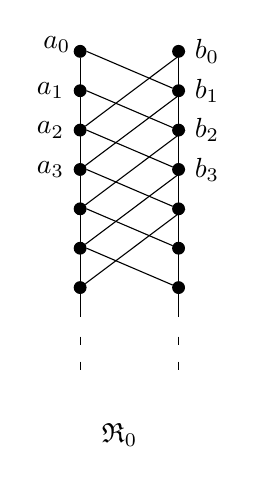
\begin{tikzpicture}[scale=0.25]
	\pgfmathsetmacro{\NODESIZE}{1.5pt}
	
	-- draw left column of nodes
	\foreach \y in {0,...,6}{
		\node[draw,circle, inner sep=\NODESIZE,fill] (leftnode \y) at (0,2*\y) {};
	}
	-- add two invisible nodes for the descending line at infinity
	\node[draw=none] (leftend1) at  (0,-2) {};
	\node[draw=none] (leftend2) at  (0,-5) {};
	
	-- draw right column of nodes
	\foreach \y in {0,...,6}{
		\node[draw,circle, inner sep=\NODESIZE,fill] (rightnode \y) at (5,2*\y) {};
	}
	\node[draw=none] (rightend1) at (5,-2) {};
	\node[draw=none] (rightend2) at (5,-5) {};
	
	-- draw the ladder itself
	\foreach \y in {0,...,4}{
		\pgfmathparse{\y+2}
		\draw [-] (leftnode \y) to (rightnode \pgfmathresult);
	}
	\foreach \y in {0,...,5}{
		\pgfmathparse{\y+1}
		\draw [-] (rightnode \y) to (leftnode \pgfmathresult);
	}
	
	--construct the vertical bars and descend into infinity
	\draw [-] (leftnode 6) to (leftend1);
	\draw [loosely dashed] (leftend1) to (leftend2);
	\draw [-] (rightnode 6) to (rightend1);
	\draw [loosely dashed] (rightend1) to (rightend2);
	

	-- label the fuckers    
	\node [left] at (leftnode 6.north)  {$a_0$};
	\node [left] at (leftnode 5.west)  {$a_1$ };
	\node [left] at (leftnode 4.west)  {$a_2 $};
	\node [left] at (leftnode 3.west)  {$a_3$};
	\node [right] at (rightnode 6.east) {$b_0$};
	\node [right] at (rightnode 5.east)  {$b_1$};
	\node [right] at (rightnode 4.east)  {$b_2$};
	\node [right] at (rightnode 3.east)  {$b_3$};
	
	-- caption trick
	\node[draw=none] (label) at  (2,-7) {};
	\node [] at (label.south)  {$\fR_0$};
	\end{tikzpicture} %\captionof{figure}{A caption.}
	\hspace{0.6cm}% NO SPACE!
		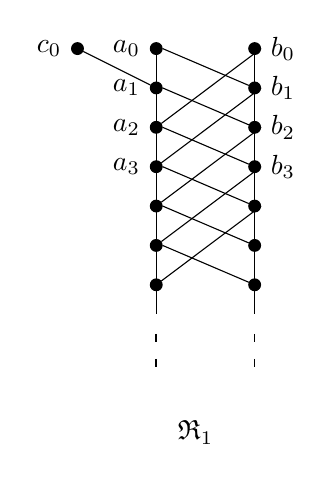
\begin{tikzpicture}[scale=0.25]
		\pgfmathsetmacro{\NODESIZE}{1.5pt}
		
		-- draw left column of nodes
		\foreach \y in {0,...,6}{
			\node[draw,circle, inner sep=\NODESIZE,fill] (leftnode \y) at (0,2*\y) {};
		}
		-- add two invisible nodes for the descending line at infinity
		\node[draw=none] (leftend1) at  (0,-2) {};
		\node[draw=none] (leftend2) at  (0,-5) {};
		
		-- draw right column of nodes
		\foreach \y in {0,...,6}{
			\node[draw,circle, inner sep=\NODESIZE,fill] (rightnode \y) at (5,2*\y) {};
		}
		\node[draw=none] (rightend1) at (5,-2) {};
		\node[draw=none] (rightend2) at (5,-5) {};
		
		-- draw the ladder itself
		\foreach \y in {0,...,4}{
			\pgfmathparse{\y+2}
			\draw [-] (leftnode \y) to (rightnode \pgfmathresult);
		}
		\foreach \y in {0,...,5}{
			\pgfmathparse{\y+1}
			\draw [-] (rightnode \y) to (leftnode \pgfmathresult);
		}
		
		--construct the vertical bars and descend into infinity
		\draw [-] (leftnode 6) to (leftend1);
		\draw [thick, loosely dashed] (leftend1) to (leftend2);
		\draw [-] (rightnode 6) to (rightend1);
		\draw [loosely dashed] (rightend1) to (rightend2);
		
		--add the branching to the left node
		\node[draw,circle, inner sep=\NODESIZE,fill] (leftmost) at (-4,12) {};
		\draw [] (leftnode 5) to (leftmost);
		
		-- label the fuckers    
		\node [left] at (leftnode 6.west)  {$a_0$};
		\node [left] at (leftnode 5.west)  {$a_1$ };
		\node [left] at (leftnode 4.west)  {$a_2 $};
		\node [left] at (leftnode 3.west)  {$a_3$};
		\node [left] at (leftmost.west)  {$c_0$};
		\node [right] at (rightnode 6.east) {$b_0$};
		\node [right] at (rightnode 5.east)  {$b_1$};
		\node [right] at (rightnode 4.east)  {$b_2$};
		\node [right] at (rightnode 3.east)  {$b_3$};
		
		-- caption trick
		\node[draw=none] (label) at  (2,-7) {};
		\node [] at (label.south)  {$\fR_1$};
		\end{tikzpicture} 
	\hspace{0.6cm}% NO SPACE!
		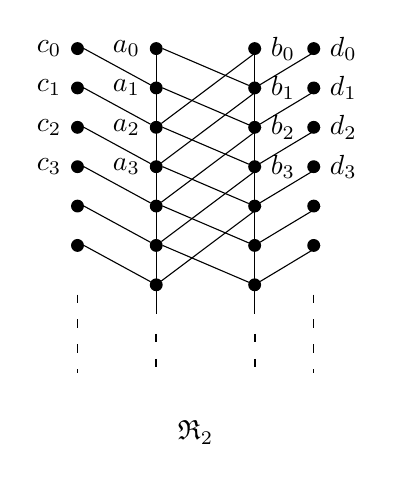
\begin{tikzpicture}[scale=0.25]
		\pgfmathsetmacro{\NODESIZE}{1.5pt}
		
		-- draw left column of nodes
		\foreach \y in {0,...,6}{
			\node[draw,circle, inner sep=\NODESIZE,fill,yshift=0em] (leftnode \y) at (0,2*\y) {};
		}
		-- add two invisible nodes for the descending line at infinity
		\node[draw=none] (leftend1) at  (0,-2) {};
		\node[draw=none] (leftend2) at  (0,-5) {};
		
		-- draw right column of nodes
		\foreach \y in {0,...,6}{
			\node[draw,circle, inner sep=\NODESIZE,fill] (rightnode \y) at (5,2*\y) {};
		}
		\node[draw=none] (rightend1) at (5,-2) {};
		\node[draw=none] (rightend2) at (5,-5) {};
		
		-- draw 2right column of nodes
		\foreach \y in {1,...,6}{
			\node[draw,circle, inner sep=\NODESIZE,fill] (2rightnode \y) at (8,2*\y) {};
		}
		\node[draw=none] (2rightend1) at (8,0) {};
		\node[draw=none] (2rightend2) at (8,-5) {};
		
		
		-- draw center column of nodes
		\foreach \y in {1,...,6}{
			\node[draw,circle, inner sep=\NODESIZE,fill] (centernode \y) at (-4,2*\y) {};
		}
		\node[draw=none] (centerend1) at (-4,0) {};
		\node[draw=none] (centerend2) at (-4,-5) {};
		
		
		
		-- draw the ladder itself
		\foreach \y in {0,...,4}{
			\pgfmathparse{\y+2}
			\draw [-] (leftnode \y) to (rightnode \pgfmathresult);
		}
		\foreach \y in {0,...,5}{
			\pgfmathparse{\y+1}
			\draw [-] (rightnode \y) to (leftnode \pgfmathresult);
		}
		\foreach \y in {0,...,5}{
			\pgfmathparse{\y+1}
			\draw [-] (leftnode \y) to (centernode \pgfmathresult);
		}
		
		\foreach \y in {0,...,5}{
			\pgfmathparse{\y+1}
			\draw [-] (rightnode \y) to (2rightnode \pgfmathresult);
		}
		
		--construct the vertical bars and descend into infinity
		\draw [-] (leftnode 6) to (leftend1);
		\draw [thick, loosely dashed] (leftend1) to (leftend2);
		\draw [-] (rightnode 6) to (rightend1);
		\draw [thick, loosely dashed] (rightend1) to (rightend2);
	%	\draw [loosely dashed] (centernode 6) to (centerend1);
		\draw [loosely dashed] (centerend1) to (centerend2);
		\draw [loosely dashed] (2rightend1) to (2rightend2);
		
		-- label the fuckers    
		\node [left] at (leftnode 6.west)  {$a_0$};
		\node [left] at (leftnode 5.west)  {$a_1$ };
		\node [left] at (leftnode 4.west)  {$a_2 $};
		\node [left] at (leftnode 3.west)  {$a_3$};
		\node [right] at (rightnode 6.east) {$b_0$};
		\node [right] at (rightnode 5.east)  {$b_1$};
		\node [right] at (rightnode 4.east)  {$b_2$};
		\node [right] at (rightnode 3.east)  {$b_3$};
		\node [left] at (centernode 6.west) {$c_0$};
		\node [left] at (centernode 5.west)  {$c_1$};
		\node [left] at (centernode 4.west)  {$c_2$};
		\node [left] at (centernode 3.west)  {$c_3$};
		\node [right] at (2rightnode 6.east) {$d_0$};
		\node [right] at (2rightnode 5.east)  {$d_1$};
		\node [right] at (2rightnode 4.east)  {$d_2$};
		\node [right] at (2rightnode 3.east)  {$d_3$};
		-- caption trick
		\node[draw=none] (label) at  (2,-7) {};
		\node [] at (label.south)  {$\fR_2$};
		\end{tikzpicture}\caption{Rieger-Nishimura Style Ladders}	
		\label{rieger-nishimura}
\end{figure}
	
	
\noindent We remark that by our previous observation an equivalent sufficient and necessary characterisation of regular Esakia spaces can be proved in exactly the same way for the subclass of Esakia spaces dual to finitely generated Heyting algebras.

Next, we can use the relation $\sim_\infty$ defined in this section to supplement \cref{maximalinjectivity} and characterise p-morphisms preserving polynomials of regulars between finite posets.
	
	\begin{proposition}\label{preservation-polynomials}
	Let $h:\fF\to\fF'$ be a p-morphism between finite posets, then $h$ preserves polynomials of regulars if and only if  $x\nsim_{\infty} y$ entails $f(x)\nsim_{\infty}f(y)$.
	\end{proposition}
	\begin{proof} 
		$(\Rightarrow)$ Suppose $h:\fF\to\fF'$ is a p-morphism preserving polynomials of regular elements, and let  $x\nsim_{\infty} y$. Since $h$ preserves polynomials of regulars, the induced map $ h^{-1}: \langle \mathcal{UR}(\fF) \rangle \to \langle \mathcal{UR}(\fF')\rangle$ is an isomorphism of Heyting algebras. It follows that $x\in h^{-1}(U)$ and $y\notin h^{-1}(U)$ for some $h^{-1}(U)\in  \mathcal{UR}(\fF)$.  Hence, we obtain that $h(x)\in U$ and $h(y)\notin U$ for some $U\in  \mathcal{UR}(\fF)$, which by \cref{lemmaquotient2} proves our claim. $(\Leftarrow)$ The other direction is analogous.
	\end{proof}
	
	We conclude this section with two side 	results on the behaviour of the quotient operations that we have introduced. Firstly, the next proposition shows  that the sequence of quotients by $\sim_n$ does not in general need to converge to any finite value.
	
	\begin{proposition}\label{dna-rieger}
	There is a compact poset $\fF$ such that each $\fF/\sim_{n}$ is distinct, for each $n<\omega$.
	\end{proposition}
	\begin{proof}
	Consider the poset $\fR_1$ in \cref{rieger-nishimura}, originally defined in \cite{Quadrellaro.2019}. It is readily verified that for every $n<\omega$, $a_n\nsim_{n+1}a_{n+1}$. Therefore, for every $n<m<\omega$ we have that $\fF/\sim_{n}$ and $\fF/\sim_{m}$ are distinct. \qedhere
	\end{proof}

	It is natural to consider what is the intermediate logic of all regular compact posets. To this end, we start by considering the Rieger-Nishimura ladder $\fR_0$ in \cref{rieger-nishimura}. One can notice that, by adding one maximal element, it is possible to obtain the Rieger-Nishimura ladder as a p-morphic image of the regular compact poset $\fR_1$. As a matter of fact, it was proven already in \cite[Cor. 5.2.3]{Ciardelli.2009} that  $S(\ipc^\neg)=\ipc$, which by \cite[Prop. 4.17]{bezhanishvili_grilletti_quadrellaro_2022} means that the variety generated by regular Heyting algebras is the whole variety of Heyting algebras.
	
	In the light of this result, one may wonder what happens if, instead of looking at regularity, we restrict attention to strongly regular posets. We say that a Heyting algebra is strongly regular if its dual Esakia space is strongly regular.  The next theorem establishes that the variety generated by the class of strongly regular Heyting algebras  is the whole variety of Heyting algebras. To show this result, it suffices to prove that any (finite) Kripke frame can be obtained as a p-morphic image of a (finite) strongly regular one. The key point is to construct, given a specific poset, a new compact poset which is strongly regular and which has the original poset as a p-morphic image. Before providing the details of this construction, we believe it is useful to illustrate the underlying idea with an example.
	
	Consider the Rieger-Nishimura ladder, we construct in  \cref{rieger-nishimura} the poset $\fR_2$, which we call the \textit{strong regularisation} of $\fR_0$. Since each $c_i$ and $d_i$ from $\fR_2$ is maximal, it is then easy to verify that different elements from $\fR_2$ see different maximal elements. The map $p:\fR_2\to \fR_0$ defined by letting, for each $i<\omega$, $p(a_i)=a_i$, $p(b_i)=b_i$, $p(c_i)=a_0$ and $p(d_i)=b_0$ is thus a p-morphism from a strongly regular poset onto the Rieger-Nishimura lattice. We generalize this construction to arbitrary posets.
	
	\begin{definition}
		Let $\fF$ be a compact poset, the \textit{strong regularisation} of $\fF$ is the poset $\fF^*$ obtained by adding, for each element $x\in \fF$, a new maximal element $x^*$ such that $(x^*)^\downarrow=x^\downarrow\cup \{x^*\}$.
	\end{definition}
	
	\noindent It is then possible to prove that any finite Kripke frame is a p-morphic image of its strong regularisation, hence showing that strongly regular Heyting algebras generate the whole variety of Heyting algebras.
	
	\begin{theorem}
		The variety generated by strongly regular Heyting algebra is $\HA$.
	\end{theorem}
	\begin{proof}
		Since the logic of the class of all finite posets is $\ipc$, it suffices to show that every (finite) poset is a p-morphic image of a finite strongly regular poset. To this end, let $\fF$ be an arbitrary finite poset and $\fF^*$ be its strong regularisation. Clearly $\fF^*$ is also finite. Let $p:\fF^*\to\fF$ be defined by letting $p(x)=x$ for all $x\in \fF$, and $p(x^*)\in M(x)$ for all $x^*\in \fF^*\setminus\fF$, i.e. $p$ assigns each $x^*$ to some maximal element that it “chooses” from $M(x)$. We check that $p$ is a p-morphism.
		\begin{itemize}
			\item[(i)] \textit{Forth Condition:} If $x\leq y$ for $x,y\in \fF$ then obviously $p(x)\leq p(y)$. If $x\leq y^*$ then $x\leq y$ and thus	$p(x)\leq p(y)\leq p(y^*)$.
			
			\item[(ii)] \textit{Back Condition:} If $p(x^*)\leq y$ then since $p(x^*)$ is maximal we immediately have $y=p(x^*)$. Otherwise, if $p(x)\leq y$  and $x\in \fF$, then we have that $p(x)\leq y=p(y)$.
		\end{itemize}
		\noindent This shows that $p:\fF^*\to \fF$ is a p-morphism, which completes our proof.		
	\end{proof}

	\section{Cardinality of $\Lambda(\HA^{\uparrow})$} \label{cardinality.sublattice}
	
	In this section we apply the characterisation of regular posets of \cref{sec.characterisation} to show that the lattice of $\dna$-varieties $\Lambda(\HA^{\uparrow})$  and the lattice of $\dna$-logics $\Lambda(\ipc^\neg)$  have power continuum. This solves a question raised in \cite{Quadrellaro.2019,bezhanishvili_grilletti_quadrellaro_2022} and complements the previous result that the sublattice of $\dna$-logics extending $\inqB$ is dually isomorphic to $\omega+1$. Inquisitive logic has thus a special location in the lattice of negative variants, having only countably many extensions. 
	
	In \cref{jankov_formulas} we recall the notion of Jankov's formulae for the setting of $\dna$-varieties as it was developed in \cite{bezhanishvili_grilletti_quadrellaro_2022} and we explain how they can be used to prove that there exist continuum-many  $\dna$-varieties of Heyting algebras. Then, in \cref{antichain0,antichain1}, we use the results from \cref{sec.characterisation} to show that two standard examples of collections of finite posets are dual to regularly generated Heyting algebras. It is then straightforward to conclude that the size of $\Lambda(\HA^{\uparrow})$  and  $\Lambda(\ipc^\neg)$ is $2^{\aleph_0}$.
	
	\subsection{Jankov's Formulae}\label{jankov_formulas} To prove the uncountability of  $\Lambda(\HA^{\uparrow})$ we adapt to our setting the notion and the method of Jankov's formulae. 	Jankov's formulae were introduced in \cite{Jankov.1963, Jankov.1968} in order to show that the lattice of intermediate logic has the cardinality of the continuum. We recall how to adapt Jankov's formulae to the setting of $\dna$-logics and $\dna$-varieties. The following definitions and results are from \cite{bezhanishvili_grilletti_quadrellaro_2022}.
	
	
 	\begin{definition}
	Let $H\in \HArfsi $, let $0$ be the least element of $H$ and $s$ its second greatest element.
 	\begin{itemize}
 	    \item The \textit{Jankov representative} of $x\in H$ is a formula $\psi_x$ defined as follows:
 		\begin{itemize}
 			\item[(i)] If $x\in H_\neg$, then $\psi_x=p_x$, where $p_x\in\at$;
 			
 			\item[(ii)] If $x=\delta_H(a_0,...,a_n)$ with $a_0,...,a_n\in H_\neg$, then $\psi_x=\delta(p_{a_0},...,p_{a_n})$.
 		\end{itemize}
 	    
 	    \item  The \textit{Jankov $\dna$-Formula} $\chi^{\dna}(H)$ is defined as follows:	
 		$$\chi^{\dna}(H):= \alpha \rightarrow \psi_s,$$
 		\noindent where $\alpha$ is the following formula:
 		 		\begin{align*}
    \alpha= (\psi_0\leftrightarrow \bot) \; \land \; &\bigwedge \{(\psi_a\land \psi_b) \leftrightarrow \psi_{a\land b}\mid a,b\in H    \} \; \land \\
 		 &\bigwedge \{(\psi_a\lor \psi_b) \leftrightarrow \psi_{a\lor b}\mid a,b\in H  \} \; \land \\
 		  &\bigwedge \{(\psi_a\rightarrow \psi_b) \leftrightarrow \psi_{a\rightarrow b}\mid a,b\in H  \}.
 		\end{align*}
 	\end{itemize}
 	\end{definition}
 	
 	\noindent As it is generally clear from the context that we are dealing with the $\dna$-version of Jankov's formulae, we write just $\chi(H)$ for the Jankov $\dna$-formula of $H$.   We recall the following result from \cite[Thm. 4.31]{bezhanishvili_grilletti_quadrellaro_2022}. For any $A,B\in \HA$, we write $ A\leq B $ if $A\in \mathbb{HS}(B) $.
 
 	\begin{theorem}\label{JT}
 		Let $A\in \HArfsi$ and $B\in \HA$ then $B\nvDash^\neg \chi(A) \text{ iff } A\leq B.$
 	\end{theorem}
	
	\noindent The next proposition adapts to the context of $\dna$-logics Jankov's classical result on intermediate logics and Heyting algebras.
	
	\begin{proposition}\label{antichain.jankov}
	Let $\cC$ be an $\leq$-antichain of finite, regular, subdirectly irreducible Heyting algebras, then for all $\mathcal{I},\mathcal{J}\subseteq \cC$ such that $\mathcal{I}\neq \mathcal{J}$ we have that $Log^\neg(\mathcal{I})\neq Log^\neg(\mathcal{J})$.
	\end{proposition}
	\begin{proof}
	Since $\mathcal{I}\neq \mathcal{J}$ there is without loss of generality some $H\in\mathcal{I}\setminus \mathcal{J}$. By Theorem $\ref{JT}$ it follows that $H\nvDash^\neg \chi(H)$, thus $\chi(H)\notin Log^\neg(\mathcal{I})$. Since $\cC$ is an antichain, $H\nleq K$ for all $K\in \mathcal{J}$, which by Theorem \ref{JT} gives $K\vDash^\neg \chi(H)$, whence $\chi(H)\in Log^\neg(\mathcal{I})$.
	\end{proof}
	
	 To prove that the lattice of $\dna$-logics has power continuum it is thus sufficient  to exhibit an infinite antichain of finite, regular, subdirectly irreducible Heyting algebras. Perhaps surprisingly, we can use examples of antichains which are standard in the literature, as they turn out to consist of regularly generated algebras. 
	
	\subsection{Antichain $\Delta_0$}\label{antichain0} We start by introducing the antichain $\Delta_0$---for this example see e.g. \cite[p. 71]{bezhanishvili2006lattices}. This is an  antichain of posets which are all regular, but which, as we shall see, contains for all $n<\omega$ infinitely many elements which are not stable under $\sim_n$. For every $n<\omega$ we define the poset $\fF_n$, with domain	
	\[  \dom(\fF_n)=\{ r\} \cup \{a_m \mid   m\leq n \} \cup \{b_m \mid  m\leq n \} \cup \{c_m \mid  m\leq n \};  \]
	\noindent and such that
	\begin{itemize}
		\item $r\leq a_i, b_i, c_i \text{ for all } i\leq n;$
		\item $a_i\leq a_j, a_i\leq b_j \text{ and } c_i\leq c_j, c_i\leq b_j \text{ whenever } j\leq i;$
		\item $b_i\leq a_j \text{ and } b_i\leq c_j \text{ whenever } j\leq i.$
	\end{itemize}
	\begin{figure}
		\begin{center}
	    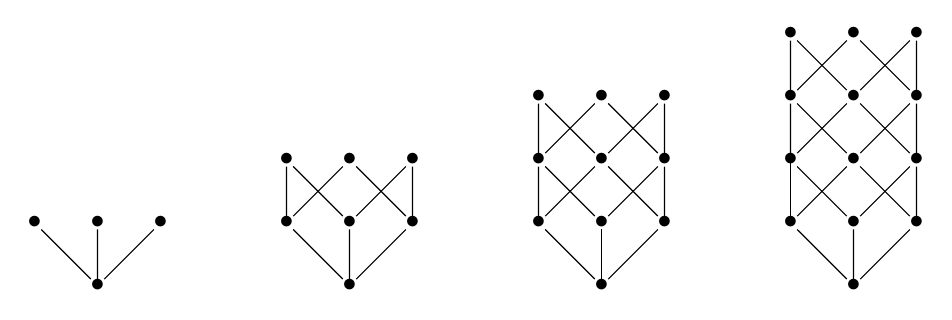
\begin{tikzpicture}[scale=0.8]
		\node[inner sep=0pt] (0)    at ( -8,0) {$\bullet$};
		\node[inner sep=0pt] (00)  at (-9,1) {$\bullet$};
		\node[inner sep=0pt] (01)  at (-8,1) {$\bullet$};
		\node[inner sep=0pt] (10)  at (-7,1) {$\bullet$};
		
        \draw (0)  -- (00);
		\draw (0)  -- (10);
		\draw (0)  -- (01);
	    
	    %----
	    \node[inner sep=0pt] (u)    at ( -4,0) {$\bullet$};
		
		\node[inner sep=0pt] (x0)  at (-5,1) {$\bullet$};
		\node[inner sep=0pt](x1) at ( -5,2) {$\bullet$};
		
		\node[inner sep=0pt](y0)  at (-4,1) {$\bullet$};
		\node[inner sep=0pt](y1) at ( -4,2) {$\bullet$};
		
		\node[inner sep=0pt](z0)  at (-3,1) {$\bullet$};
		\node[inner sep=0pt](z1) at ( -3,2) {$\bullet$};

        \draw (u)    -- (x0);
		\draw (u)    -- (y0);
		\draw (u)    -- (z0);

		\draw (x0)    -- (x1);
		%\draw (y0)    -- (y1);
		\draw (z0)    -- (z1);
		\draw (x0)    -- (y1);
		\draw (y0)    -- (z1);
		\draw (y0)    -- (x1);
		\draw (z0)    -- (y1);
	    
	    
	    %-----
	    
		\node[inner sep=0pt](p)    at ( 0,0) {$\bullet$};
		
		\node[inner sep=0pt](d0)  at (-1,1) {$\bullet$};
		\node[inner sep=0pt](d1) at ( -1,2) {$\bullet$};
		\node[inner sep=0pt](d2)  at (-1,3) {$\bullet$};
		
		\node[inner sep=0pt](e0)  at (0,1) {$\bullet$};
		\node[inner sep=0pt](e1) at ( 0,2) {$\bullet$};
		\node[inner sep=0pt](e2)  at (0,3) {$\bullet$};
		
		\node[inner sep=0pt](f0)  at (1,1) {$\bullet$};
		\node[inner sep=0pt](f1) at ( 1,2) {$\bullet$};
		\node[inner sep=0pt](f2)  at (1,3) {$\bullet$};

        \draw (p)    -- (d0);
		\draw (p)    -- (e0);
		\draw (p)    -- (f0);

		\draw (d0)    -- (d1);
		\draw (d1)    -- (d2);
		
		%\draw (e0)    -- (e1);
		%\draw (e1)    -- (e2);
		
		\draw (f0)    -- (f1);
		\draw (f1)    -- (f2);
		
		\draw (e0)    -- (d1);
		\draw (e1)    -- (d2);
		
		\draw (e0)    -- (f1);
		\draw (e1)    -- (f2);
		
		\draw (d0)    -- (e1);
		\draw (d1)    -- (e2);
		
		\draw (f0)    -- (e1);
		\draw (f1)    -- (e2);
		
		%-----
		
		\node[inner sep=0pt](p)    at ( 4,0) {$\bullet$};
		
		\node[inner sep=0pt](d0)  at (3,1) {$\bullet$};
		\node[inner sep=0pt](d1) at ( 3,2) {$\bullet$};
		\node[inner sep=0pt](d2)  at (3,3) {$\bullet$};
		\node[inner sep=0pt](d3)  at ( 3,4) {$\bullet$};
		
		\node[inner sep=0pt](e0)  at (4,1) {$\bullet$};
		\node[inner sep=0pt](e1) at ( 4,2) {$\bullet$};
		\node[inner sep=0pt](e2)  at (4,3) {$\bullet$};
		\node[inner sep=0pt](e3)  at (4,4) {$\bullet$};
		
		\node[inner sep=0pt](f0)  at (5,1) {$\bullet$};
		\node[inner sep=0pt](f1) at ( 5,2) {$\bullet$};
		\node[inner sep=0pt](f2)  at (5,3) {$\bullet$};
		\node[inner sep=0pt](f3)  at (5,4) {$\bullet$};

        \draw (p)    -- (d0);
		\draw (p)    -- (e0);
		\draw (p)    -- (f0);

		\draw (d0)    -- (d2);
		\draw (d1)    -- (d2);
		\draw (d2)    -- (d3);
		
		%\draw (e0)    -- (e1);
		%\draw (e1)    -- (e2);
		%\draw (e2)    -- (e3);
		
		\draw (f0)    -- (f1);
		\draw (f1)    -- (f2);
		\draw (f2)    -- (f3);
		
		\draw (e0)    -- (d1);
		\draw (e1)    -- (d2);
		\draw (e2)    -- (d3);
		
		\draw (e0)    -- (f1);
		\draw (e1)    -- (f2);
		\draw (e2)    -- (f3);
		
		
		\draw (d0)    -- (e1);
		\draw (d1)    -- (e2);
		\draw (d2)    -- (e3);
		
		\draw (f0)    -- (e1);
		\draw (f1)    -- (e2);
		\draw (f2)    -- (e3);
		
        %---
		
		%\node[inner sep=0pt](dots1)    at ( 6,0) {$\dots$};
%		\node[inner sep=0pt](dots2)    at ( 7,1) {$\dots$};	
%		\node[inner sep=0pt](dots3)    at ( 7,2) {$\dots$};
%		\node[inner sep=0pt](dots4)    at ( 7,3) {$\dots$};
		%\node[inner sep=0pt](dots5)    at ( 6,4) {$\dots$};
	\end{tikzpicture}
	\caption{The Antichain $\Delta_0$}	
	\label{Delta0}
	
\end{center}
\end{figure}

	
	\noindent We let $\Delta_0:=\{ \fF_n \mid  n<\omega  \}$ be the set of all such posets. The following result follows by noticing that we cannot perform neither $\alpha$ nor $\beta$-reductions on any $\fF_n$ without collapsing the maximal elements---we refer the reader to \cite[Lem. 3.4.19]{bezhanishvili2006lattices} for a proof.
	
	\begin{proposition}\label{antichain.1}
	The set of Heyting algebras dual to $\Delta_0$ is a $\leq$-antichain. 
	\end{proposition}
	
	\noindent Since every poset in $\Delta_0$ is finite and rooted, it follows immediately by Esakia duality that its algebraic duals are finite, subdirectly irreducible, Heyting algebras. In order to establish our result we  also need to make sure that every Heyting algebra which we are dealing with is regularly generated. This follows from the characterisation of finite regular posets which we provided in  \cref{sec.characterisation}. We recall that, if $\fF$ is a finite poset, then the \textit{depth} of an element $x\in \fF$, written $\depth(x)$, is defined as the size of the maximal chain in $x^\uparrow\setminus\{x\}$. Clearly the depth of a maximal elements is 0 and, in each $\fF_n$ the depth of the root is $n+1$.
	
	\begin{proposition}\label{antichain.regularity}
	    For every $n<\omega$, the Kripke frame $\fF_n$ is regular. In particular,  $\fF_n/\sim_n=\fF_n$ for every $n<\omega$.
	\end{proposition}
	\begin{proof}
	Consider $\fF_n$ for some $n<\omega$, we prove by induction on $\depth(x)$ that $[x]_k = \{x \}  $ whenever $k\geq \depth(x)-1$, for $\depth(x)>0$ and $k\geq 0$ otherwise.
	\begin{itemize}
	    \item Let $\depth(x)\leq 1$. Without loss of generality we let $x=a_{1}$. Then, given any $y\in \fF_n$ such that $y\neq a_1$, we clearly have $M(a_1)\neq M(y)$, showing $[a_1]_0=\{a_1\}$.
	    
	    \item Let $\depth(x)=m+1< n+1$.  Without loss of generality we let $x=a_{m+1}$ and by induction hypothesis $[a_{l}]_{k}=\{a_{l}\}$, $[b_{l}]_{k}=\{b_{l}\}$ and $[c_{l}]_{k}=\{c_{l}\}$ whenever $l\leq k+1$, $l \leq m$. Now, for all $y\in \fF_n$ such that $x\neq y$, if $\depth(y)\leq m$ then $[y]_{m}=\{y\}$, thus  $[y]_{k}=\{y\}$  for all $k\geq m$. Otherwise, if $\depth(y)>m$ then since $y\neq a_{m+1}$, it follows $y\leq c_{m}$, proving $x\nsim_{m}y$ and thus $x\nsim_{k}y$ for all $k\geq m$. It follows $[x]_{k} =\{x\}$ for all $k\geq m=\depth(x)-1$.
	    
	    \item Let $\depth(x)=n+1$.The only point with depth $n+1$ in $\fF_n$ is the root $r$ and clearly it is the only point in $[r]_{n}$.
	\end{itemize}
	\noindent It follows that  $[x]_n=\{x\}$ for all $x\in \fF_n$ and thus $\fF_n/\sim_n =\fF_n$.
	\end{proof}
	
	\noindent We often call \emph{n-regular} a poset $\fF$ such that $\fF=\fF/\sim_n$. 
	
	Once we know that every poset from the antichain $\Delta_0$ above is regular, it is then straightforward to reason as in Jankov's original proof and show that the cardinality of the lattices of $\dna$-logics and $\dna$-varieties is exactly $2^{\aleph_0}$. We say that a finite Heyting algebra has \emph{width} (or \emph{depth}) $n$ if its dual poset has width (or depth) $n$,
	
	\begin{theorem}\label{continuum.logics}
	There are continuum-many $\dna$-logics and $\dna$-varieties. In particular, there are continuum-many $\dna$-varieties generated by Heyting algebras of width 3.
	\end{theorem}
	\begin{proof}
	Let $\cA_0$ be the set of Heyting algebras dual to the posets in $\Delta_0$. Since every poset in $\Delta_0$ has width 3, the same holds for the dual Heyting algebras. By \cref{antichain.1}, $\cA_0$ is an infinite $\leq$-antichain of finite, subdirectly irreducible Heyting algebras. Moreover, by \cref{characterisation.regular} and \cref{antichain.regularity} we also have that each Heyting algebra in $\cA_0$ is regularly generated. By Theorem \ref{antichain.jankov} we have $Log^\neg(\mathcal{I})\neq Log^\neg(\mathcal{J})$ whenever $\mathcal{I},\mathcal{J}\subseteq \Delta_0$ and $\mathcal{I}\neq \mathcal{J}$. By duality, we also have $Var^\neg(\mathcal{I})\neq Var^\neg(\mathcal{J})$ whenever $\mathcal{I},\mathcal{J}\subseteq \Delta_0$ and $\mathcal{I}\neq \mathcal{J}$. Since $|\Delta_0|=\omega$, our result follows immediately.
	\end{proof}
	
	\noindent We also remark that, given the fact that $\dna$-varieties are in one-to-one correspondence with varieties of Heyting algebras generated by regular algebras, this also shows the existence of continuum-many varieties of Heyting algebras generated by regular elements. 
	
	\subsection{Antichain $\Delta_1$}\label{antichain1}	Interestingly, we can also apply another standard example of infinite $\leq$-antichain to our context, originally due to Kuznetsov \cite{kuznetsov}, and show that there are continuum-many subvarieties of Heyting algebras which are generated by strongly regular elements.  
	
	We recall the following construction and redirect the reader to \cite[\S 3]{bezhanishvili2022jankov} for more details. For every $2<n<\omega$, we let $\fG_n$ be the partial order with domain
	\[  \dom(\fG_n)=\{ r\} \cup \{a_m \mid m\leq n \} \cup \{b_m\mid m\leq n \}  \]
	\noindent and such that
	\begin{itemize}
		\item $r\leq a_i, b_i, \text{ for all } i<n;$
		\item $a_0\leq b_j,  \text{ for all } 0\leq j< n;$
		\item $a_n\leq b_j,  \text{ for all } 0<j\leq  n;$
		\item $a_i\leq b_j, \text{ if } 0<i<n \text{ and } i\neq j.$
	\end{itemize}

	\noindent We let $\Delta_1:=\{ \fG_n\mid 2<n<\omega  \}$ be the set of all such posets. One can check that, whenever we collapse two maximal points in a frame $\fG_{n+1}$, the result is that every point of depth 1 is related to every point of depth 0, which is not the case in $\fG_n$. We thus obtain the following proposition, whose detailed proof is left to the reader.
	
	\begin{proposition}\label{antichain.2}
	The set of Heyting algebras dual to $\Delta_1$ is a $\leq$-antichain. 
	\end{proposition}

		
	\begin{figure}
		\begin{center}
			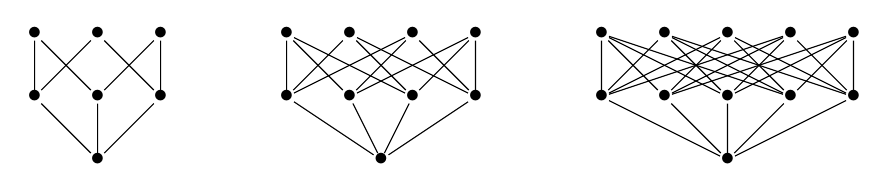
\begin{tikzpicture}[scale=0.8]
			
			\node[inner sep=0pt](u)    at ( -5,0) {$\bullet$};
			
			\node[inner sep=0pt](x0)  at (-6,1) {$\bullet$};
			\node[inner sep=0pt](x1) at ( -6,2) {$\bullet$};
			
			\node[inner sep=0pt](y0)  at (-5,1) {$\bullet$};
			\node[inner sep=0pt](y1) at ( -5,2) {$\bullet$};
			
			\node[inner sep=0pt](z0)  at (-4,1) {$\bullet$};
			\node[inner sep=0pt](z1) at ( -4,2) {$\bullet$};
			
			\draw (u)    -- (x0);
			\draw (u)    -- (y0);
			\draw (u)    -- (z0);
			
			\draw (x0)    -- (x1);
			\draw (z0)    -- (z1);
			\draw (x0)    -- (y1);
			\draw (y0)    -- (z1);
			\draw (y0)    -- (x1);
			\draw (z0)    -- (y1);			
			%-----
			
			\node[inner sep=0pt](p)    at ( -0.5,0) {$\bullet$};
			
			\node[inner sep=0pt](d0)  at (-2,1) {$\bullet$};
			\node[inner sep=0pt](d1) at ( -1,1) {$\bullet$};
			\node[inner sep=0pt](d2)  at (0,1) {$\bullet$};
			\node[inner sep=0pt](d3)  at (1,1) {$\bullet$};
			
			\node[inner sep=0pt](e0)  at (-2,2) {$\bullet$};
			\node[inner sep=0pt](e1) at ( -1,2) {$\bullet$};
			\node[inner sep=0pt](e2)  at (0,2) {$\bullet$};
			\node[inner sep=0pt](e3)  at (1,2) {$\bullet$};
			
			\draw (p)    -- (d0);
			\draw (p)    -- (d1);
			\draw (p)    -- (d2);
			\draw (p)    -- (d3);
			
			\draw (d0)    -- (e0);
			\draw (d0)    -- (e1);
			\draw (d0)    -- (e2);
			
			\draw (d3)    -- (e3);
			\draw (d3)    -- (e1);
			\draw (d3)    -- (e2);
			
			\draw (d2)    -- (e3);
			\draw (d2)    -- (e1);
			\draw (d2)    -- (e0);
			
			\draw (d1)    -- (e3);
			\draw (d1)    -- (e2);
			\draw (d1)    -- (e0);
			
			%-----
			\node[inner sep=0pt](m)    at ( 5,0) {$\bullet$};
			
			\node[inner sep=0pt](m0)  at (3,1) {$\bullet$};
			\node[inner sep=0pt](m1) at ( 4,1) {$\bullet$};
			\node[inner sep=0pt](m2)  at (5,1) {$\bullet$};
			\node[inner sep=0pt](m3)  at (6,1) {$\bullet$};
			\node[inner sep=0pt](m4)  at (7,1) {$\bullet$};
			
			\node[inner sep=0pt](n0)  at (3,2) {$\bullet$};
			\node[inner sep=0pt](n1) at ( 4,2) {$\bullet$};
			\node[inner sep=0pt](n2)  at (5,2) {$\bullet$};
			\node[inner sep=0pt](n3)  at (6,2) {$\bullet$};
			\node[inner sep=0pt](n4)  at (7,2) {$\bullet$};
			
			\draw (m)    -- (m0);
			\draw (m)    -- (m1);
			\draw (m)    -- (m2);
			\draw (m)    -- (m3);
			\draw (m)    -- (m4);
			
			\draw (m0)    -- (n0);
			\draw (m0)    -- (n1);
			\draw (m0)    -- (n2);
			\draw (m0)    -- (n3);
			
			\draw (m4)    -- (n4);
			\draw (m4)    -- (n1);
			\draw (m4)    -- (n2);
			\draw (m4)    -- (n3);
			
			\draw (m3)    -- (n0);
			\draw (m3)    -- (n1);
			\draw (m3)    -- (n2);
			\draw (m3)    -- (n4);
			
			
			\draw (m2)    -- (n3);
			\draw (m2)    -- (n1);
			\draw (m2)    -- (n0);
			\draw (m2)    -- (n4);
			
			\draw (m1)    -- (n3);
			\draw (m1)    -- (n2);
			\draw (m1)    -- (n0);
			\draw (m1)    -- (n4);
			
			%---
%			\node[inner sep=0pt](dots2)    at ( 9,1) {$\dots$};
			\end{tikzpicture}
			\caption{The Antichain $\Delta_1$}	
			\label{Delta1}
		\end{center}
	\end{figure}
	
	
		
	
	\noindent As the posets in $\Delta_1$ grow in width rather than depth, we have that every $\fG_n$ is stable already under the quotient $\sim_0$, i.e. $\fG_n/\sim_0=\fG_n$ for all $2<n<\omega$. So every poset in $\Delta_1$ is actually strongly regular.
	
	\begin{proposition}\label{antichain.regularity.2}
		Every poset $\fG_n$ is strongly regular.
	\end{proposition}
	\begin{proof}
		By construction, it is straightforward to check that any two different $x,y\in \fG_n$ see different maximal elements, i.e. $M(x)\neq M(y)$.
	\end{proof}
	
	\noindent By the same reasoning as above, we immediately obtain a second uncountable family of $\dna$-varieties and $\dna$-logics.
	
	\begin{theorem}
	There are continuum many $\dna$-varieties generated by strongly regular Heyting algebras of depth 3.
	\end{theorem}
	\begin{proof}
	Analogously to \cref{continuum.logics}, together with the fact that posets from $\Delta_1$ are strongly regular and have depth 3.
	\end{proof}

	\noindent In particular, this also means that there are continuum-many variety of Heyting algebras generated by strongly regular elements.

	\section{Connections to Dependence Logic}\label{dependence.logic}
	In this last section we conclude by pointing out some connections between the topics previously discussed and (propositional) dependence logic. 
	
	Dependence logic was introduced by V\"a\"an\"anen \cite{Vaananen2007-VNNDLA} as an extension of first-order logic with dependence atoms. A key aspect of dependence logic is that it is formulated in so-called \textit{team-semantics}, which was originally introduced by Hodges in \cite{Hodges}. In its propositional version, which was developed by Yang and V\"a\"an\"anen in \cite{Yang2016-YANPLO,Yang2017-YANPTL}, teams are simply sets of propositional assignments. It was soon observed in Yang's thesis \cite{yang2014extensions} -- see also in \cite{Ciardelli2016,Yang2016-YANPLO} -- that the team semantics of propositional logic actually coincides with the state-based  semantics of inquisitive logic, thus establishing an important connection between dependence and inquisitive logic, which has later been object of several investigations.
	
	In this section we shall explore a further aspect of this connection and we will illustrate the relation between propositional dependence logic and regular Heyting algebras. In particular, we will adapt the completeness proof of \cref{algebraic.completeness.dna} so as to obtain a sound and complete topological semantics for dependence logic.
	
	
	\subsection{Syntax and Semantics}
	
	Dependence logic can be seen as an extension of inquisitive logic in a larger vocabulary $\langInqI$, which adds the so-called tensor operator to the signature of intuitionistic logic. Dependence logic can be thus presented in the following syntax $\langInqI$:
\begin{align*}
\phi ::= p \mid  \bot   \mid  \phi \land \phi \mid \phi\otimes \phi \mid \phi \lor \phi \mid \phi\rightarrow\phi.
\end{align*}
	
\noindent We define $\neg\alpha:=\alpha\to\bot$ and we say that a formula is \textit{standard} if it does not contain any instance of $\lor$. We provide this syntax with the usual team semantics. We recall that a propositional \textit{assignment} (also \textit{valuation}) is a map $w:\at\to 2$ and that a \textit{team} is a set of assignments $t\in \wp( 2^\at)$. The team semantics of dependence logic is then defined as follows. 

\begin{definition}[Team Semantics]
	The notion of a formula $\phi\in\langInqI$ being \textit{true in a team} $t\in \wp({2^\at})$ is defined as follows: 
	
	\begin{equation*}
	\begin{array}{l @{\hspace{1em}\Longleftrightarrow\hspace{1em}} l}
	t\vDash p & {}\forall w\in t \ ( w(p)=1)  \\
	t\vDash \bot &  t=\varnothing \\
	t\vDash \psi \lor \chi & t\vDash \psi \text{ or } t\vDash \chi\\
	t\vDash \psi \land \chi & t\vDash \psi \text{ and } t\vDash \chi\\
	t\vDash \psi \otimes \chi & \exists s,r\subseteq t \text{ such that } s\cup r = t \text{ and } s\vDash \psi, r\vDash \chi \\
	t\vDash \psi \rightarrow \chi &  \forall s \ ( \text{if }s\subseteq t \text{ and } s\vDash\psi \text{ then } s\vDash \chi ).
	\end{array}
	\end{equation*}
\end{definition}

\noindent  We define \emph{propositional dependence logic} as the system  $\inqB^\otimes= Log( \wp(2^\at))$ of all formulas of $\langInqI$ valid under team semantics. We notice that inquisitive logic has exactly the same semantics but it is formulated in the restricted language $\langInt$, which lacks the tensor disjunction, whence we clearly have that $\inqB^\otimes\supseteq \inqB$.

We also remark that the propositional dependence atom can be defined in this system as follows:
\[ \dep (p_0,\dots, p_n, q):= \bigwedge_{i\leq n} (p_i\lor \neg p_i ) \to (q\lor \neg q). \]

\noindent We thus notice that, despite the name, it is not the dependence atom which distinguishes the propositional version of inquisitive and dependence logics, but rather the presence of the tensor. This observation is also justified by the work of Barbero and Ciardelli in  \cite{ciardelli2019undefinability}, as they showed that the tensor cannot be uniformly defined by the other operators. 

\subsection{Algebraic Semantics of Dependence Logic} As we have recalled above, inquisitive logic admits a (non-standard) algebraic semantics, which was introduced in \cite{grilletti} and further investigated in \cite{bezhanishvili_grilletti_quadrellaro_2022}. As dependence logic extends inquisitive logic by the tensor operator, it is natural to provide it with an algebraic semantics by augmenting inquisitive algebras with an interpretation for it. Such a semantics was first introduced in \cite{quadrellaro2021intermediate} and was later shown in  \cite{nakov.quadrellaro} to be unique up to a suitable notion of algebraizability. We can use such algebraic semantics to build a bridge with Esakia spaces and provide a topological semantics for dependence logic. Firstly, we introduce the notion of $\inqB^\otimes$-algebras as in \cite{nakov.quadrellaro}.

\begin{definition}
	An \emph{$\inqB^\otimes$-algebra} $A$ is a structure in the signature $\langInqI$ such that: 
	\begin{enumerate}
	    \item $A{ \restriction } \{\lor,\land,\to, \bot  \} \in Var(\mathtt{ML})  $;
	    \item $A_\neg{ \restriction } \{\otimes,\land,\to, \bot  \} \in \BA$;
	    \item $A \vDash x \otimes (y \lor z) \approx (x\otimes y) \lor (x\otimes z);$
	    \item $A \vDash (x\to z) \to (y \to k) \approx  (x\otimes y) \to (z\otimes k).$
	\end{enumerate}
\end{definition}

\noindent Hence, an $\inqB^\otimes$-algebra is the expansion of  a Heyting algebra satisfying the validities of $\mathtt{ML}$, and the additional conditions above.  By expanding the previous definition, one can see that it amounts to the equational definition of a class of algebras, thus giving rise to a variety of structures. Notice that, as the regular elements of a Heyting algebra always form a Boolean algebra, what the condition $\cA_\neg{ \restriction } \{\otimes,\land,\to, \bot  \} \in \BA$ really entails is that, for all regular elements $x,y\in \cA_\neg$, $x\otimes y := \neg(\neg x \land \neg y)$, i.e. the tensor is the “real” Boolean disjunction over regular elements. 


We let $ \mathsf{InqBAlg^\otimes} $ be the variety of all $\inqB^\otimes$-algebras and  we write $ \mathsf{InqBAlg^\otimes_{FRSI}} $ for its subclass of finite, regular and subdirectly irreducible elements. We say that $A$ is a \emph{dependence algebra} if it belongs to the subvariety generated by all finite, regular, subdirectly irreducible $\inqB$-algebras, i.e. if $A\in \mathbb{V}(\mathsf{InqBAlg^\otimes_{FRSI}})$. We write $\mathsf{DA}:= \mathbb{V}(\mathsf{InqBAlg^\otimes_{FRSI}})$ for the variety of dependence algebras. It was proven in  \cite{nakov.quadrellaro} that $\mathsf{DA}$ is the equivalent algebraic semantics of $\inqB^\otimes$. In particular, we have the following completeness result:

\begin{theorem}[Algebraic Completeness]\label{algebraic.complete.dependence}
	For any formula $\phi\in \langInqI$ we have that  $\phi \in \inqB^\otimes$ if and only if $ \mathsf{DA}  \vDash^\neg \phi$.
\end{theorem}

\noindent In particular, we notice that on the right hand side we are using the same notion of truth of \cref{subsection:dnaLogicsAndAlgebraicSemantics}, i.e. formulas of dependence logic are evaluated under negative assignments, which map atomic formulas to regular elements of the underlying dependence algebra. 


\subsection{Topological Semantics of Dependence Logic} 
The algebraic semantics of propositional dependence logic makes for an important bridge with the topological approach that we developed in this article. By the very definition of dependence algebra we have that they are Heyting algebras (more specifically $\mathtt{ML}$-algebras), whence we can dualize them according to Esakia duality. The only problem arising when proceeding in this way is that, as the Esakia duality  accounts only for the Heyting algebra structure of a dependence algebra, the correct interpretation of the tensor operator is “lost in translation”. To avoid this problem we shall consider only regularly generated dependence algebras.

Let $\fE$ be a regular  Esakia space satisfying $\mathtt{ML}$, it is easy to provide an interpretation for the tensor product over clopen upsets $\fE$. In fact, as we remarked previously, the tensor operator is the Boolean dual of conjunction with respect to regular elements. Moreover, since regular $\mathtt{ML}$-Esakia spaces are also inquisitive, it follows immediately from  \cref{regular.inquisitive} that any clopen upset of a regular $\mathtt{ML}$-Esakia space is a union of regular ones. This allows us to define the tensor operator over $\mathcal{CU}(\fE)$ as follows:
\begin{enumerate}
    \item For  $U,V\in \mathcal{RCU}(\fE)$ we let $U\otimes V := \overline{(\overline{U} \cup \overline{V})}$;
    \item For  $U,V\in \mathcal{CU}(\fE)\setminus \mathcal{RCU}(\fE)$ we let \[U\otimes V := \bigcup \{ U_0 \otimes V_0\mid  U_0\subseteq U, V_0\subseteq V, U_0,V_0\in  \mathcal{RCU}(\fE) \}.\]
\end{enumerate}

\noindent We leave it to the reader to verify that $\mathcal{CU}(\fE)$ forms a dependence algebra, where the tensor operator is interpreted as we remarked. However, although this definition suffices in explaining how the tensor can be interpreted over algebras of clopen upsets, it still does not provide us with a topological intuition of its behaviour. To this end, we prove the following proposition. 

\begin{proposition}\label{tensor.description}
Let $\fE$ be a regular Esakia space satisying $\mathtt{ML}$, and let $\otimes$ be defined by the clauses above, then we have, for any $U,V\in \CU(\fE)$: 
\begin{align*}
	x\in U\otimes V \Longleftrightarrow  \; & M(x)\subseteq U_0\cup V_0 \\\; &\text{for some } U_0\subseteq U \text{ and } V_0\subseteq V \text{ such that } U_0,V_0\in \mathcal{C}(M_\fE).
\end{align*}
\end{proposition}
\begin{proof}
Firstly, if  $U,V\in \mathcal{RCU}(\fE)$ we have by definition $U\otimes V = \overline{(\overline{U} \cup \overline{V})}$. We obtain:
    \begin{align*}
        x\in \overline{(\overline{U} \cup \overline{V})} &\Longleftrightarrow  \forall y\geq x, \; y\notin \overline{U} \cap \overline{V} \\
        &\Longleftrightarrow  \forall y\geq x \; \exists z \geq y, \; z\in U \cup V \\
        &\Longleftrightarrow M(x)\subseteq U \cup V\\
        &\Longleftrightarrow M(x)\subseteq M(U) \cup M(V).
    \end{align*}
\noindent Then, for arbitrary  $U,V\in \mathcal{CU}(\fE)$, the claim follows immediately from the definition of the tensor and the induction hypothesis.
\end{proof}

\noindent The previous proposition thus provides us with a topological interpretation for the tensor operator and shows that the tensor disjunction between two clopen upsets of an Esakia space is uniquely determined by the Stone subspace of its maximal elements. 

 Now, let $\mathsf{Esa^{\mathtt{ML}}_{RFR}}$ be the class of rooted, finite and regular posets which satisfy $\mathtt{ML}$ -- we  described this class in greater details  in \cref{strongly.regular.inquisitive}. Then by the definition of the variety of dependence algebras, it follows that the validity of $\inqB^\otimes$-formulas is always witnessed by finite, regularly generated, subdirectly irreducible algebras (see also \cite{quadrellaro2021intermediate}). The following theorem thus follows exactly as \cref{algebraic.completeness.dna}, by applying Esakia duality and  interpreting the tensor as we illustrated above. 

\begin{theorem}[Topological Completeness]\label{topological.complete.dependence}
	For any formula $\phi\in \langInqI$ we have that  $\phi \in \inqB^\otimes$ if and only if $ \mathsf{Esa^{\mathtt{ML}}_{RFR}} \vDash^\neg \phi$.
\end{theorem}

This last result shows that propositional dependence logic admits a topological semantics, where the tensor operation can be described as in \cref{tensor.description}. As the validity of formulas is preserved by the variety operations, we can extend the previous result and infer the completeness of $\inqB^\otimes$ with respect to the closure of the class $\mathsf{Esa^{\mathtt{ML}}_{RFR}}$ under subspaces, disjoint unions and p-morphisms. Notice, however, that our topological characterisation of the tensor operator is limited to regular Esakia spaces. The questions whether the tensor admits an interesting topological interpretation also in non-regular spaces, or whether the previous construction can be meaningfully adapted to regular posets which are not strongly regular, should be subject of further investigations.

	\section{Conclusion}\label{conclusion}

	In this article we have considered regular Heyting algebras from the point of view of Esakia duality, and we have provided several results about their dual topological spaces. 
	
	In \cref{topological.semantics} we have reviewed some folklore results on the connection between an  Esakia space and its Stone subspace of maximal elements. Using this fact we have adapted to Esakia spaces the algebraic semantics of inquisitive and $\dna$-logics.
	
	In \cref{sec.characterisation} we have focused on the main problem of the article, i.e. the characterisation of (finite) regular Esakia spaces. In \cref{morphism.characterisation} we spelled out the natural dual characterisation of regular Heyting algebras in terms of p-morphisms, and we refined this characterisation for finite posets using $\alpha$- and $\beta$-reductions. In \cref{quotient.characterisation} we followed another strategy and we introduced a family of equivalence relations over compact posets, i.e. posets where every element sees a maximal element. We used these notions to provide a necessary criterion for an arbitrary Esakia space to be regular and also to give a further characterisation of finite, regular posets. Such quotients also allowed us to provide a more fine-grained study of regular posets, and to identify for example the subfamily of strongly regular posets.
	
	We gave an example of application of these characterisations in  \cref{cardinality.sublattice}, where  we showed that there are continuum many varieties of Heyting algebras generated by (strongly) regular posets. In particular, this means that there are continuum many $\dna$-logics, in contrast to the fact that there are only countably many extensions of inquisitive logic.
	
	Finally, in \cref{dependence.logic}, we reviewed the well-known connection between dependence and inquisitive logic, and we applied the results of the present article to propositional dependence logic. Analogously to what we did for $\dna$-logics, we proved a topological completeness result for dependence logic, and we gave a topological description of the tensor disjunction over regular Esakia spaces.
	
	We believe that the present work hints at some possible directions of further research. Besides the points already raised in the article, we wish here to bring three points to attention. 
	
	Firstly, in \cite{quadrellaro2021intermediate} we have considered the algebraic semantics of a wide range of intermediate versions of inquisitive and dependence logics. As this semantics relies on Heyting algebras with a core of join-irreducible elements, it is then natural to ask to what extent one could extend the duality results of this article to this context.
	
	Secondly, is it possible to extend our characterisation of finite regular posets from \cref{quotient.characterisation} to account also for infinite Esakia spaces? As we have briefly remarked, the case of Esakia spaces which are dual to finitely generated Heyting algebras does not pose serious problems, but in general this seems a non-trivial matter, as the notion of regularity is purely order-theoretic and independent from the Esakia topology. Interestingly, this also relates to the problem of the Esakia representability of (compact) posets studied in \cite{BEZHANISHVILI2021107959}. 
	
	Finally, the class of regular compact posets has a quite combinatorial nature and makes for an interesting class of structures. Is it possible to provide a model-theoretic classification of these structures? Can we describe, for instance, all finite ($n$-)regular posets up to some notion of dimension, e.g. their depth or their number of maximal elements? We leave these and other problems to future research. 
	
	
	
	\printbibliography
	

\end{document}


